%% main_ppgco_ufu.tex v1.0, Lásaro Camargos e Denise Guliato
% adaptado de modeloABNT2.tex, v1.0 athila 
% ------------------------------------------------------------------------
% ------------------------------------------------------------------------
% eesc: Modelo de Trabalho Acadêmico (tese de doutorado, dissertação de
% mestrado e trabalhos monográficos em geral) em conformidade com 
% ABNT NBR 14724:2011. Esta classe estende as funcionalidades da classe
% abnTeX2 elaborada de forma a adequar os parâmetros exigidos pelas 
% normas USP e do departamento de elétrica da Escola de Engenharia 
% de São Carlos - USP.
% ------------------------------------------------------------------------
% ------------------------------------------------------------------------

% ------------------------------------------------------------------------
% Opções:
% 	tesedr:     Formata documento para tese de doutorado
%	qualidr:    Formata documento para qualificação de doutorado
% 	dissertmst: Formata documento para dissertação de mestrado
% 	qualimst:   Formata documento para qualificação de mestrado
% ------------------------------------------------------------------------
\documentclass[dissertgrad,oneside]{tcc}
%Não altere o comando seguinte. O título de seu trabalho será especificado mais adiante.
\title{Trabalho de Conclusão de Curso}

% ---
% PACOTES
% ---

% ---
% Pacotes fundamentais 
% ---
\usepackage{cmap}				% Mapear caracteres especiais no PDF
\usepackage{lmodern}				% Usa a fonte Latin Modern			
\usepackage{makeidx}            	% Cria o indice
\usepackage{hyperref}  			% Controla a formação do índice
\usepackage{lastpage}			% Usado pela Ficha catalográfica
\usepackage{indentfirst}			% Indenta o primeiro parágrafo de cada seção.
\usepackage{nomencl} 			% Lista de simbolos
\usepackage{graphicx}			% Inclusão de gráficos
\usepackage{datetime}
% ---

% ---
% Pacotes adicionais, usados apenas no âmbito do Modelo eesc
% ---
\usepackage{lipsum}				       % para geração de dummy text
\usepackage[printonlyused]{acronym}
\usepackage[table]{xcolor}
\usepackage{listings}
\usepackage{amsmath}
\usepackage{indentfirst}
\usepackage{color}
\usepackage{cite}
\usepackage{pdflscape}
% ---

% ---
% Informações de dados para CAPA e FOLHA DE ROSTO
% ---
%
% Título:
%	1. Título em português
%	2. Título em inglês
\titulo{Framework para Controle de Sistemas Industriais via MQTT}{Industrial Automation Framework MQTT}
%
% Autor:
%	1. Nome completo do autor
%	2. Formato de nome para bibliografia
\autor{Thiago de Souza Alves }{Alves, Thiago}
%
% Cidade
\local{Uberlândia}
% Ano de defesa
\data{\the\year{}}
% Área de concentração da pesquisa
\areaconcentracao{Engenharia Mecatrônica}
% Nome do orientador
\orientador{José Jean-Paul Zanlucchi Souza Tavares}
% Nome do coorientador
% ---

% ---
% compila o indice
% ---
\makeindex
% ---

% ---
% Compila a lista de abreviaturas e siglas
% ---
\makenomenclature
% ---

% ---
% Inserir ficha catalográfica
%
% Caso o comando \inserirfichacatalografica seja definido, a %ficha catalográfica
% será inserida atrás da folha de rosto. Caso contrário a página será deixada em
% branco.
%
% CUIDADO: Esta opção deve ser preenchida antes do comando \maketitle
% ---
%entre em contato com a biblioteca para obter a sua ficha catalográfica em arquivo pdf. Essa %folha só será inserida no documento após a sua defesa.

\inserirfichacatalografica{fichaCatalografica.pdf}
% ---

% ---
% Inserir folha de aprovação
%
% Caso o comando \inserirfolhaaprovacao seja definido, a folha de aprovação
% será inserida. Além disso, conforme Resolução CoPGr 5890, as informações 
% de rodapé são inseridas apropriadamente na folha de rosto.
%
% CUIDADO: Esta opção deve ser preenchida antes do comando \maketitle
% ---
% baseie-se no modelo desse documento e gere a sua folha de %rosto em arquivo pdf.

\inserirfolhaaprovacao{folhaAprovacao.pdf}
% ---

% ----
% Início do documento
% ----

\begin{document}

% ----------------------------------------------------------
% ELEMENTOS PRÉ-TEXTUAIS
% ----------------------------------------------------------
\pretextual

% ---
% Insere Capa, Folha de rosto, Ficha catalográfica (se inserida)
% e folha de aprovação (se inserida).
% ---
\maketitle


% ---
% Dedicatória
% ---
\imprimirdedicatoria{Este trabalho é dedicado aos meus pais,\\
os primeiros a me ensinar que as coisas tem um porque de acontecer, \\
a crença mais louca e inexplicável que nos faz humanos, \\
que insiste em permanecer viva apesar das constantes provas contrárias.}
% ---

% ---
% Agradecimentos
% ---
\imprimiragradecimentos{

Agradeço também ao professor Jean-Paul, pela orientação e motivação, mostrando qual o real sentido do trabalho realizado.
E também a toda a equipe do projeto FEMEC Maker que tem feito um excelente trabalho em conjunto no sentido de desenvolver
o aparato da faculdade de Mecânica da UFU.

}
% ---

% ---
% Epígrafe
% ---
\imprimirepigrafe{
		``Sobre isto dizem os filósofos que a Natureza não faz nada em vão, e mais algo é vão quando menos serve. 
        Pois a Natureza é simples e não se compraz com causas supérfluas.''\\
		(Isaac Newton)
}
% ---

% ---
% RESUMO e ABSTRACT
% ---

% Resumo em português - as palavras entre chaves são as palavras-chave do trbalho
\begin{resumo}{MQTT, Nuvem, IOT, Comando, microcontroladores, Industria 4.0}

    Uma das linhas de desenvolvimento na Indústria 4.0 é a \ac{IOT} onde busca-se a inclusão de componentes responsáveis por 
    realizar parte do processamento em \textit{edge}, de forma a enviar para os servidores centrais da aplicação (geralmente 
    alocados em lugares especiais ou até em nuvem) somente os dados cruciais para o sistema. Um dos principais meios para a 
    concretização deste conceito é o protocolo \ac{MQTT}, pois o mesmo permite que cada objeto tenha maior autonomia para definir suas funções
    na rede.
    Neste sentido este projeto se dispõe a apresentar um modelo comunicação para inclusão de
    elementos básicos utilizados em sistemas de manufatura ao modelo \ac{IOT}; apresentando uma série de tecnologias 
    selecionadas para manter a implementação destes conceitos simples e adaptável a uma grande gama de componentes.
    Por fim, foram realizados uma série de testes em bancada eletro-hidráulica e eletro-pneumática comprovando fisicamente
    a funcionalidade do modelo e suas limitações.   

\end{resumo}

% Resumo em inglês
\begin{abstract}{MQTT, Cloud, IOT, Command, microcontrolers, Industry 4.0}

    One of development lines in Industry 4.0 is \ac{IOT} which seeks to include development of components responsible for
    perform part of the processing at the edge, sending to the main application servers (generally
    allocated in special places or even in the cloud) only the crucial data
    to the system. One of the main lines for
    implementation of this concept is \ac{MQTT} protocol, whitch allows each object to have more autonomy to define its functions
    on the network. In this sense, this project intends to present a communication model to include
    basic components used in manufacturing systems in this model; featuring a range of technologies
    selected to keep the implementation of these concepts simple and adaptable to a wide range of components.
    Finally, a series of tests were carried out on electro-hydraulic and electro-pneumatic benchs, physically proving 
    the model functionality and its limitations.
	
\end{abstract}
% ---

% ---
% inserir lista de ilustrações
% ---
\newpage
\listailustracoes
% ---

% ---
% inserir lista de tabelas
% ---
%\listatabelas
% ---

% ---
% inserir lista de abreviaturas e siglas
% ---
\listasiglas{abrev/Abreviaturas}
% ---

% ---
% inserir o sumario
% ---
\sumario
% ---

% ----------------------------------------------------------
% ELEMENTOS TEXTUAIS
% ----------------------------------------------------------
\mainmatter

% ----------------------------------------------------------
% Introdução
% ----------------------------------------------------------
\chapter[Introdução]{Introdução}

Ao estudar a história das civilizações humanas como um todo, um fato que ganha bastante evidência é a ligação próxima 
entre o desenvolvimento de novas e disruptivas técnicas e grandes transformações sociais e ecônomicas fato que pode 
ser obsevado muito claramente, nas três primeiras revoluções industriais com a inclusão, respectivamente, da máquina 
a vapor, energia elétrica e computadores gerando transformações incomensuráveis no \textit{status} social. Atualmente,
vivemos também um momento de grande transformação dirigido principalmente pelo desenvolvimento das comunicações, expondo 
ao mundo um novo nível de informações, o que, como era de se esperar, também está atrelado a uma nova revolução das 
técnicas, a indústria 4.0. Embora ela não possua ainda um componente que resuma sua importância como nas três anteriores, 
sua influência no mundo é perceptível em várias áreas: criando ambientes virtuais, comunicação entre maquinários e serviços, aumento das 
plataformas "\textit{as a service}", entre outras ramificações.

Entre os vários caminhos abertos na quarta revolução industrial, um dos mais expressivos é o da descentralização de sistemas
de grande complexidade, neste sentido o uso de componentes inteligentes capazes de resolver parte de seus desafios em 
\textit{Edge} associados a uma infraestrutura elástica\footnote{Entende-se aqui como infraestrutura elástica aquela que 
pode ser facilmente ajustada as necessidades momentâneas.} disponibilizada via nuvem tem se mostrado como uma arquitetura 
extremamente poderosa e promissora. Este trabalho, por sua vez, apresenta modo conectar componentes essenciais da manufatura
nesta arquitetura, seus ganhos e observações da aplicação prática.


\section{Motivação}
A motivação para a realização deste estudo se dá por dois grandes vieses, um deles surge pelo aumento do maquinário 
existente no \ac{MAPL} que aumenta a necessidade de um sistema que auxilie no controle e gerenciamento destes componentes
tanto de forma local como remotamente. Além disso, o grande período de afastamento dos laboratórios por conta da 
pandemia enfrentada nos últimos anos fez aumentar em muito os questionamentos sobre a necessidade de muitos processos 
essencialmente presenciais e acelerou o desenvolvimento de várias tecnologias voltadas a realização de atividades via acesso
remoto, contexto no qual este estudo se insere.

\section{Objetivos e Desafios}
O principal objetivo deste trabalho é a contrução de um modelo de comunicação, ou \textit{Framework}, que seja de simples
entendimento e possível adaptação para comunicação com outros tipos de dados, do ponto de vista de código; que seja 
modular, isto é, que possa ser adaptado a diferentes tipos de máquinários sem precisar passar por grandes alterações;
que possa ser acessado remotamente, sem que isso torne o sistema dependente de redes externas; e que, por fim, possa ser 
alterado facilmente dada a alta mutabilidade dos sistemas atuais.   

\section{Organização da Dissertação}
Seguindo os objetivos descritos acima o presente trabalho, passa pela construção de \textit{Framework} a que se impõe grande versatilidade,
desta forma durante sua construção passar-se-á por uma grande revisão de documentos normativos, manuais de fabricantes e 
documentações oficiais; pois somente assim podemos focar em quais são os limites da aplicação de suas funções diferentemente
de um trabalho onde não se sabe sobre o funcionamento e faz-se um teste para saber se funciona. Em segundo momento serão 
apresentados os conceitos que guiaram o desenvolvimento e; por fim; foi realizado uma série de testes, como uma prova de
conceito, comprovando a aplicabilidade do \textit{Framework} de forma prática.




% ----------------------------------------------------------
% Fundamentação
% ----------------------------------------------------------
\chapter[Fundamentação Teórica]{Fundamentação Teórica}

Neste capítulo serão apresentados os componentes utilizados durante o desenvolvimento do trabalho, assim como suas 
principais características e motivos de cada escolha. Componentes relacionados diretamente a montagem física do sistema
serão abordados de forma sucinta, pois o escopo do trabalho se dispões a apresentar um \textit{Framework} de desenvolvimento
que não se limita aos circuitos e componentes utilizados, por outro lado é importante pontuar alguns detalhes quanto a 
parte de implementação dos códigos que serão vitais para o entendimento da abrangência do modelo utilizado.

\section{Circuitos Eletrohidráulicos e Eletropneumáticos}

\begin{figure}[htb]
    \begin{center}
	    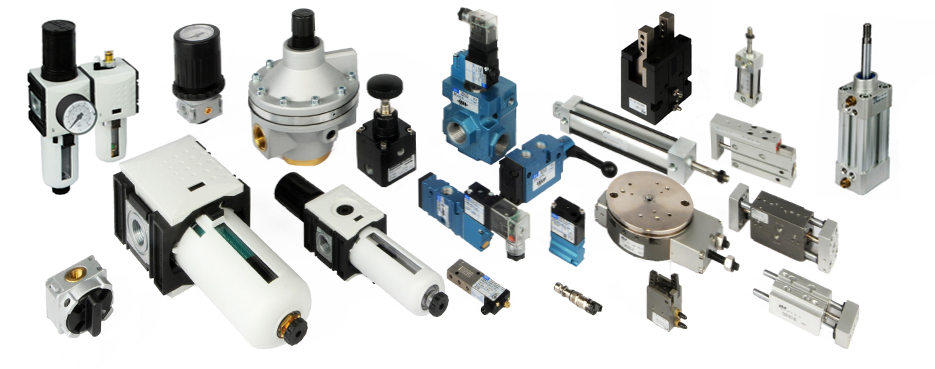
\includegraphics[scale=0.5]{figs/set-pneumatica.jpg}
	\end{center}
	\caption{Exemplo de componentes pneumáticos.} 
\end{figure}

No contexto da Engenharia Mecatrônica e da automação no geral, uma das principais tecnologias utilizadas na solução de
problemas de diferentes áreas são os circuitos de comando hidráulicos e pneumáticos, seu amplo uso já de longo período e
sua capacidade de ser implementada em diferentes campos fazem com que esta ferramenta possua ampla documentação e suporte
de uma estabelecida cadeia de suprimentos, com os mais diversos tipos de componentes. Este consolidado status garante 
que estes circuitos sejam um tópico amplamente abordado durante a formação do engenheiro, e como em qualquer outra 
ferramenta neste contexto são desenvolvidos diversos modelos e métodos que auxiliam em sua implementação. 

\subsection{Métodos de Representação e Simulação}

Uma das ferramentas mais importantes que garantem a circuitos hidráulicos e pneumáticos a posição mencionada acima é a 
existência de uma simbologia bastante sólida para os cada vez mais complexos sistemas utilizados na industria. Esta simbologia,
instituida primeiramente pela ISO 1219:1997 \cite{ISO1219:1997}, mas substituída algumas vezes logo depois até atingir a
estrutura atual, na qual seu escopo foi dividido em três partes:

\begin{figure}[htb]
    \begin{center}
	    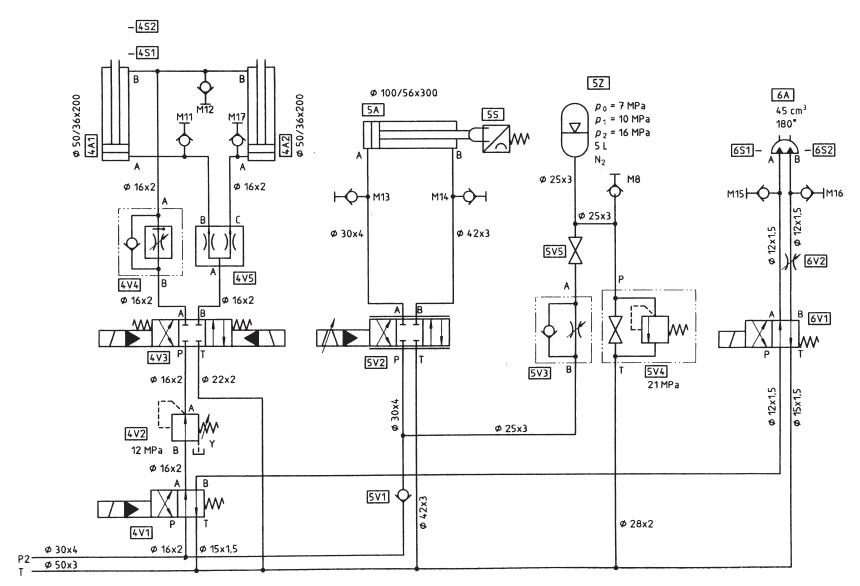
\includegraphics[scale=0.5]{figs/std-example.png}
	\end{center}
	\caption{Exemplo de diagrama proposto na norma.} 
\end{figure}

\begin{itemize}

    \item ISO 1219-1:20012 \cite{ISO1219-1:2012}: que versa diretamente sobre os símbolos utilizados nos diagramas de 
    forma isolada (esta parte recebeu em 2016 a inclusão da emenda AMD 1:2016 \cite{ISO1219-1:2012/AMD-1:2016}) 
    \item ISO 1219-2:20012 \cite{ISO1219-2:2012}: que, por sua vez, versa sobre as características construtivas de 
    circuitos conexões, agrupamento e entre outros. 
    \item ISO 1219-3:20016 \cite{ISO1219-3:2016}: que versa sobre a utilização de módulos, isto é, modelos de representação
    de pequenos agrupamentos utilizados repetitivamente em circuitos muito grandes.

\end{itemize}

A partir desta simbologia podemos criar uma série de \textit{softwares} de simulação capazes de auxiliar-nos na 
implementação dos mais diversos sistemas, como o FluidSIM\textregistered~ e o Automation Studio, onde podemos executar
versões virtuais dos ambientes reais, e observar os resultados. 

\subsection{Ladder}

Apesar do ambiente altamente robusto descrito acima, o crescimento da complexidade dos problemas abordados no meio da 
automação industrial ainda tem se mostrado como um grande desafio. Neste contexto um segundo tópico que também tem função 
importante é o desenvolvimento de métodos que pudessem auxiliar no desenvolvimento dá lógica, sendo em um primeiro momento
a inclusão dos diagramas de relés, de forma a ficarem estes componentes os principais responsáveis pelo comando; 
mas depois sendo substituído por \ac{CLP} um componente capaz de implementar via código as complicadas sequências de acionamento.
Os primeiros esforços no sentido de garantir um modelo padronizado neste sentido vieram da norma IEC 61131 que se dispunha
a trazer uma série de conceitos relacionados aos \ac{CLP}s em geral como apresentado logo no início do documento.

\begin{citacao}
    This Part of IEC 61131 applies to programmable controllers (PLC) and their associated 
    peripherals such as programming and debugging tools (PADTs), human-machine interfaces
    (HMIs), etc., which have as their intended use the control and command of machines and
    industrial processes.\cite{IEC-61131-1:2003}
\end{citacao}    

Entre todo o material apresentado na norma, a parte que mais interessa a este trabalho é a descrita na IEC 61131-3:2013 
em que são propostas quatro linguagens de programação: \ac{IL}, \ac{ST}, \ac{LD} e \ac{FBD} \cite{IEC-61131-3:2013} 
que tornavam simples a implementação de código nos \ac{CLP}s e, falando especificadamente dos códigos em \ac{LD} a 
linguagem foi construída de forma que estes códigos pudessem ser facilmente interpretados como um diagrama de relés.

\begin{citacao}
    A LD program enables the programmable controller to test and modify data by means of standardized
    graphic symbols. These symbols are laid out in networks in a manner similar to a “rung” of a relay
    ladder logic diagram. LD networks are bounded on the left and right by power rails.\cite{IEC-61131-3:2013}
\end{citacao}    

\begin{figure}[htb]
    \begin{center}
	    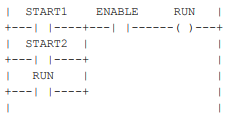
\includegraphics{figs/ladder-diag.png}
	\end{center}
	\caption{Exemplo de código Ladder proposto na norma.} 
\end{figure}

\subsection{GRAFCET}

Por fim, como último método de grande importância no desenvolvimento de circuitos hidráulicos e pneumáticos em geral, 
podemos mencionar o \ac{GRAFCET} já que este é um tipo de modelagem onde conseguimos representar de uma forma sequancial
modelos altamente complexos. Por ser baseado nas Redes de Petri o \ac{GRAFCET} é visto como um modelo com forte base
matemática comprovado pela teoria de grafos.

Apesar de ser um método para modelagem e dimensionamento de processos, alguns \ac{CLP}s aceitam o \ac{GRAFCET} como uma
linguagem de programação diretamente assim como previsto na norma IEC 60848:2013 \cite{IEC-60848:2013}, o que traz uma 
grande praticidade na implementação de processos longos, além de garantir uma maneira mais simples para entendimento dos 
processos permitindo que grandes times possam trabalhar no seu desenvolvimento.

\begin{figure}[htb]
    \begin{center}
	    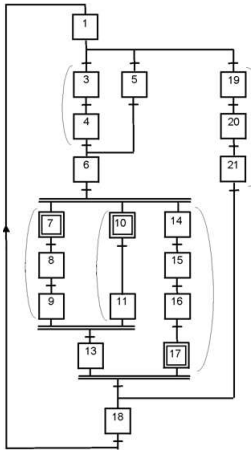
\includegraphics[scale=0.5]{figs/grafcet-diag.png}
	\end{center}
	\caption{Exemplo de código GRAFCET proposto na norma.} 
\end{figure}

\section{Computação em Nuvem}

Visto como uma das maiores \textit{buzzword}\footnote{Segundo o dicionário Cambridge: \textit{Buzzword} é uma palavra ou expressão de uma 
área de assunto particular que se tornou moda, porque tem sido muito usado \cite{buzzword-cam}} da atualidade e com uso 
ainda crescente. Porém, a definição de computação em nuvem é bastante vaga \cite{artigo-nuvem} em alguns casos sendo 
associada a virtualização de servidores, em outros casos a disponibilização de Infraestrutura como serviço (\ac{IaaS}) ou 
alguma das variações do "\textit{as a service}"; ou até em alguns casos uma referência a localização material dos grandes
\textit{Data Centers} sua disposição territorial e etc. Fato é que nem entre os próprios provedores destes serviços 
existe uma padronização, de como eles são disponibilizados; observando os três principais hoje vemos que a AWS\textregistered~
utiliza um modelo de \textit{server virtualization}, enquanto a Azure\textregistered~ se baseia no \ac{WAH} e o Google\textregistered~, por sua vez, segue o 
conceito de \textit{technique-specific sandbox} \cite{artigo-nuvem}.

No contexto deste trabalho considerar-se-á nuvem como um modelo de virtualização, no qual se delega toda a parte de 
infraestrutura computacional e podemos acessar os recursos desejados a partir de uma representação abstrata na maioria 
das vezes disponibilizadas a partir de uma interface via Internet. Conceito que apesar de gerar um grande barulho atualmente
não tem nada de novo, ao contrário, era uma dos conceitos já discutidos desde a concepção do \textit{Multics}, sistema 
operacional precursor do Unix e, portanto, do modelo seguido no GNU atual, como pode ser visto no paper de apresentação 
do projeto.

\begin{citacao}
It is important to recognize that the average user of the system will see no part of the segmentation and paging 
complexity described in the paper by Glaser et al. Instead he will see a virtual machine with many system characteristics 
which are convenient to him for writing either single programs or whole subsystems. \cite{multics-paper}
\end{citacao}

\section{O Protocolo MQTT}

Apresentado pela própria OASIS\textregistered~ como o protocolo padrão para a troca de mensagens \ac{IOT} o protocolo \ac{MQTT}
tem ganhado espaço em diversas aplicações por se mostrar como um modelo em que cada componente é capaz de controlar qual
tipo de informação ele pode transmitir e receber, o que é visto como um grande ganho do ponto de vista do \ac{IOT}; além 
disso, em uma rede \ac{MQTT} a entrada e saída de novos componentes em rede acontece de forma bastante simples, sem 
necessitar que o responsável pela rede refaça toda sua configuração.

Para implementar estes conceitos o protocolo utiliza a arquitetura \textit{publisher/subscriber} em que são definidos
uma série de tópicos e cada componente pode se cadastrar como publicador de um grupo de tópicos e subscritor de outro 
grupo de tópicos\footnote{Estes grupos não são exclusivos}. Assim, os servidores desta rede (ou \textit{Brokers} seguindo a terminologia
descrita no OASIS MQTTv5 Standard \cite{mqtt-std}) podem deixar a função de orquestradores da rede e se tornarem responsáveis
por rotear as mensagens transmitidas por cada tópico. Com o uso do \ac{MQTT}, temos um grande avanço no sentido de objetos
em rede autogerenciáveis, mais informações sobre o uso desta ferramenta em especifíco neste trabalho serão apresentadas 
mais a frente.

\begin{figure}[htb]
    \begin{center}
	    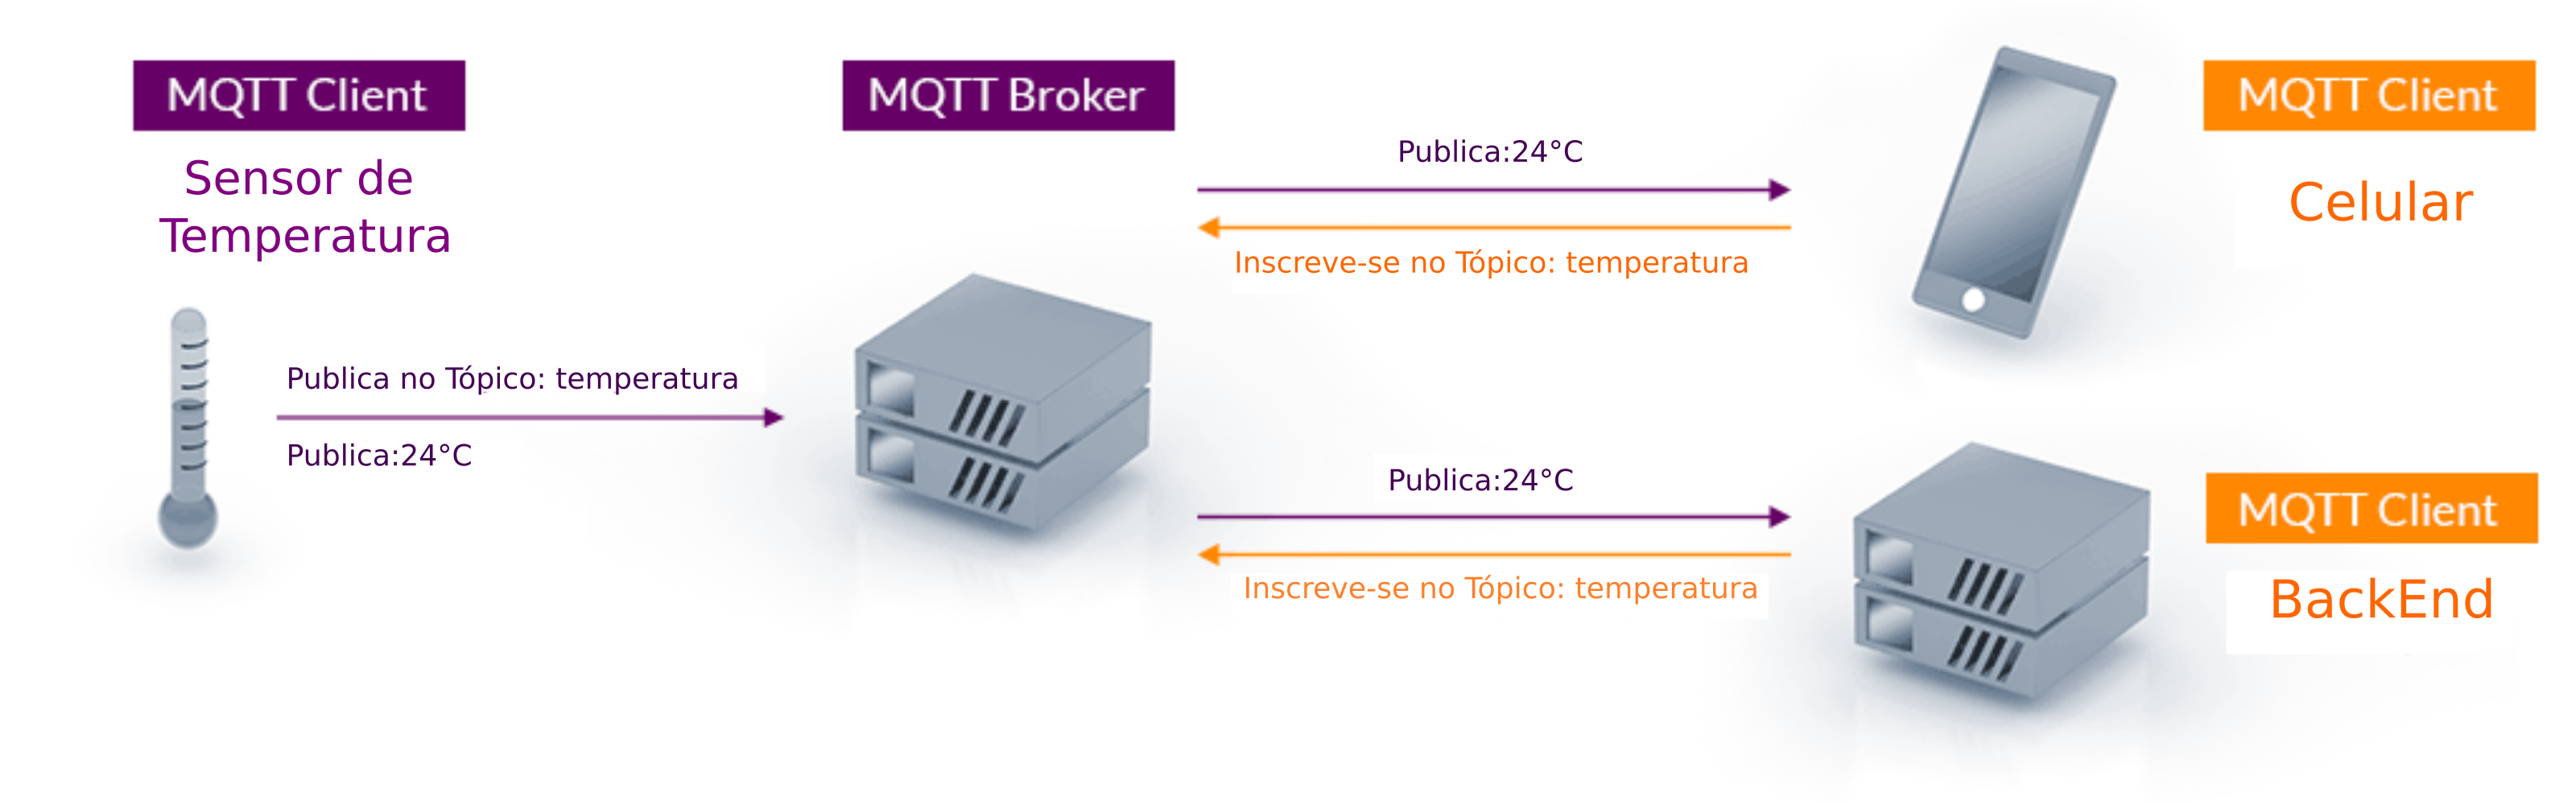
\includegraphics[scale=0.3]{figs/mqtt-publish-subscribe.png}
	\end{center}
	\caption{Diagrama representativo da arquitetura \ac{MQTT}.} 
\end{figure}

\section{Microcontroladores ESP32}

Tido como um dos principais microcontroladores para desenvolvimento \ac{IOT} os ESP tem uma grande vantagem em relação 
a uma gama de outros microcontroladores pois possuem módulos para comunicação \textit{wireless} embutidos no próprio
\textit{chip}, neste meio a família ESP32 apresenta-se, entre as linhas de produto ainda em desenvolvimento pela 
Expressif\textregistered~, como uma das mais completas apresentando como principais características:

\begin{itemize}
\item 2.4 GHz Wi­Fi + Bluetooth® + Bluetooth LE module
\item microprocessador Xtensa® dual­core 32­bit LX6
\item opções de: 4/8/16 MB memória flash
\item 26 GPIOs, com grande gama de periféricos disponíveis
\item Antena PCB na placa ou conector para antena externa
\end{itemize}

\subsection{Características do Componente}

Apesar de muitas pessoas entenderem os ESPs diretamente como uma placa de desenvolvimento, às vezes até como uma 
alternativa semelhante ao arduino, é importante fazer a distinção clara entre os dois componentes. Diferente 
do Arduino onde temos vários \ac{CI} com diferentes funções, no caso do ESP32 estamos falando de um \ac{SoC} responsável
por todas estas capacidades acima. Por outro lado, o fabricante disponibiliza em seu catálogo três modelos de encapsulamento
para o mesmo \textit{chip}, sendo eles: 

\begin{itemize}
    \item \textbf{ESP32 DOWD v3}, o próprio \ac{SoC}, sendo este o modelo mais simples e econômico para inclusão em produtos já de longo ciclo no 
    mercado, porém utilizar este componente diretamente no circuito exige um maior tempo dedicado ao \textit{design} da interface, uma 
    vez que ele traz consigo uma série de \textit{guidelines} a serem seguidos para sua instalação. \cite{datasheet-soc}
    \item \textbf{ESP32-WROOM-32E}, o módulo, sendo este o grande foco deste trabalho, é um módulo de fácil inclusão no \textit{design} de outras PCBs   
    possui já possui proteção térmica e de ruído, circuito para filtro da fonte de tensão, gerador de \textit{clock} e antena PCB inclusos. \cite{datasheet-modulo}
    \item \textbf{ESP32-DevKitC}, a placa de prototipagem, neste componente temos uma pinagem de simples acesso para as saídas do módulo de forma 
    que o uso de \textit{jumpers} fica simples, e também temos incluído botões para mudar o \textit{chip} para o modo de gravação, uma porta USB, e
    Leds indicadores de funcionamento.
\end{itemize}

\begin{figure}[htb]
    \begin{center}
	    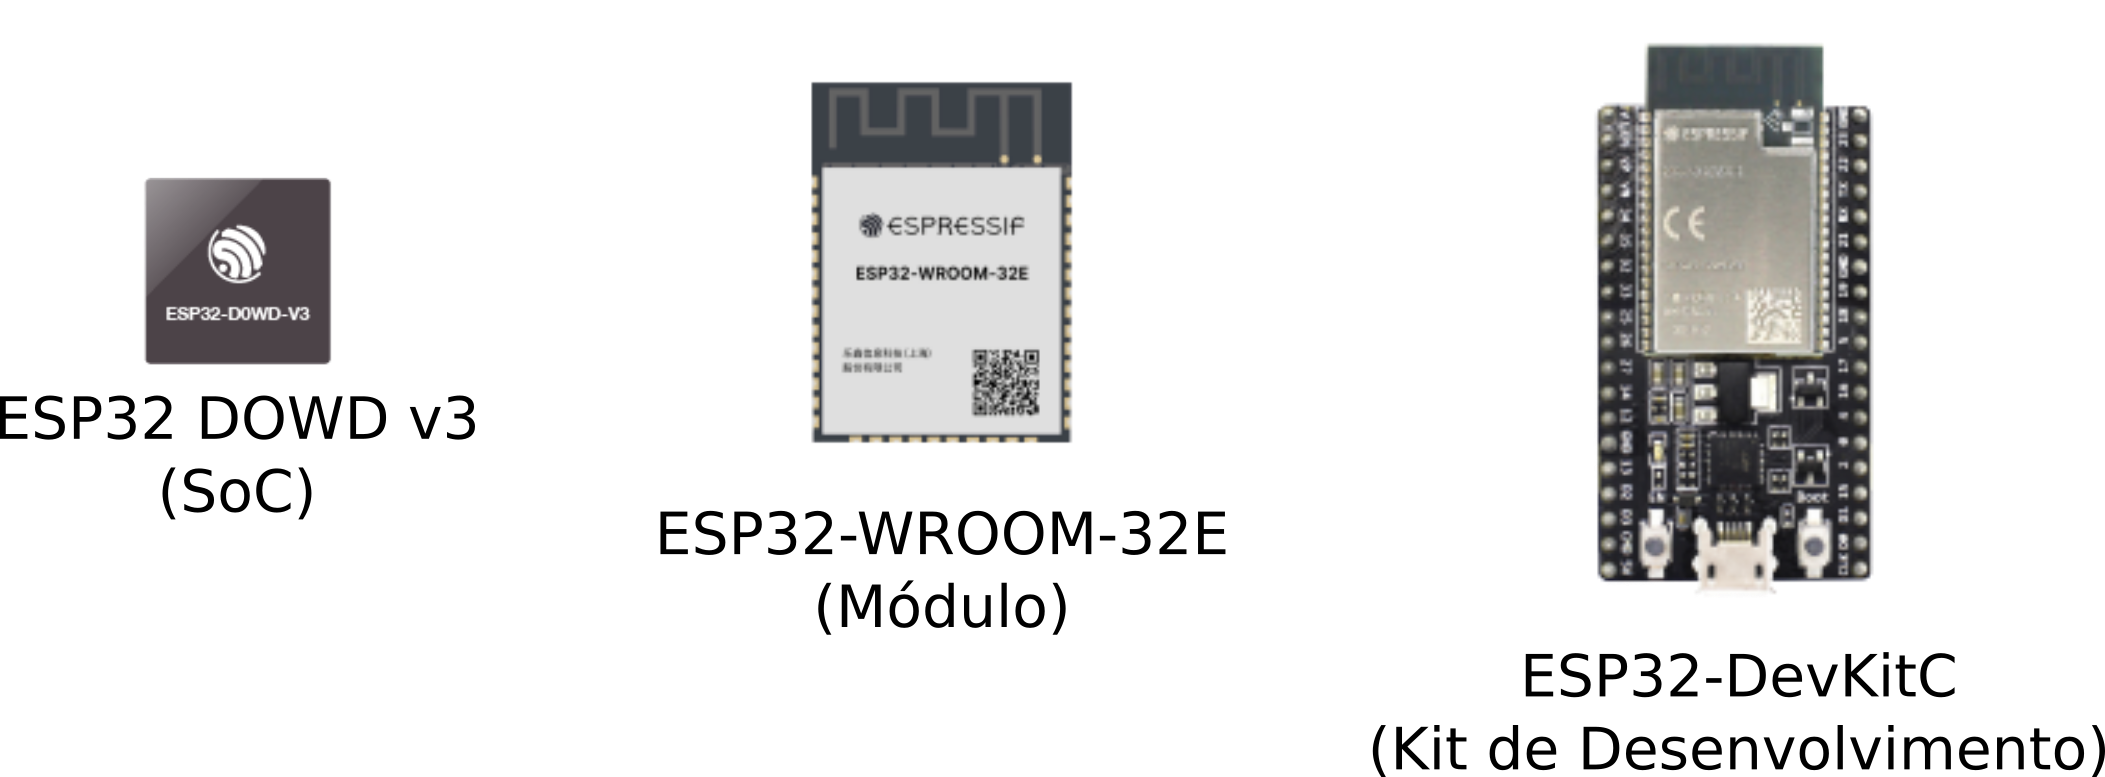
\includegraphics[scale=0.5]{figs/esp32-familia.png}
	\end{center}
	\caption{\label{fig:esp-fam} Distinção entre os componentes baseados no ESP32.} 
\end{figure}

Embora os experimentos deste trabalho tenham sido realizados com o ESP32-DevKitC, não existem restrições quanto ao seu uso também no módulo
ESP32-WROOM-32E, as representações esquemáticas destes componentes estão disponíveis respectivamente no Anexo \ref{ane:kit} e no Anexo \ref{ane:mod}.

\subsection{Ambiente de Desenvolvimento}

Outra característica importante dos ESP32 é que eles utilizam o \ac{ESP-IDF} o ambiente de desenvolvimento oficial 
disponibilizado pelo fabricante baseado \textit{FREERTOS}®. Um ambiente amplamente documentado com \textit{scripts} 
Python e Cmake que facilitam o processo de compilação e \textit{link} do \textit{firmware}, além disso do ponto de 
vista da compilação o \ac{ESP-IDF} utiliza versões oficiais do GCC com \textit{backend} específico para a a família de 
processadores Xtensa® LX6\footnote{Essa informação não abrange os ESP32-S2 ou ESP32-C3, estas séries de processadores
possuem versões diferentes do GCC (backend LX7, RISCV e etc.) assim como descrito no Github do \ac{MAPL}\cite{mapl-repo}};
e são, portanto, compatíveis com todas as linguagens suportadas no \textit{frontend} do GCC utilizado (C, C++, Objective-C,
FORTRAN, Go e etc).

\begin{figure}[htb]
    \begin{center}
	    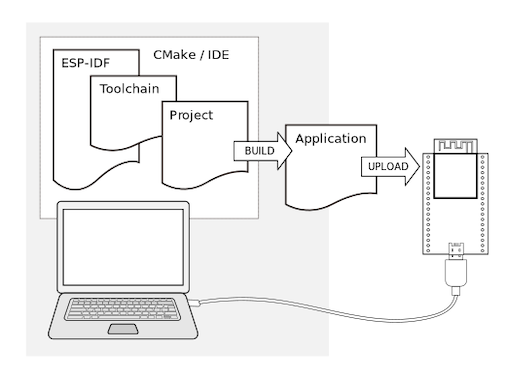
\includegraphics[scale=0.5]{figs/comp-flow.png}
	\end{center}
	\caption{Modelo \ac{ESP-IDF}.} 
\end{figure}

No momento da construção deste trabalho, a versão de suporte padrão para o \textit{framework} utilizava o GCC 5.3  com 
suporte máximo para o Std17\cite{suported-c}, assim como esperado de acordo com as informações de \textit{release} do GCC
5 \cite{gcc-5}. 

Optou-se, portanto, pela utilização em todos os códigos deste trabalho do C++17. O uso do C++ se justifica
porque o grande objetivo do trabalho é produzir uma plataforma de fácil entendimento. Por outro lado, o uso do padrão 17
se dá com o objetivo de seguir as recomendações do próprio \textit{release} disponível no site da GNU designando ente como
novo padrão para o compilador \cite{gcc-5}.


\section{A plataforma Raspberry PI\textregistered}

Uma plataforma que tem ganhado bastante notoriedade tanto nos assuntos que envolvem engenharia quanto na area da computação
são os Raspberry PI, um pouco diferente do que costuma-se ver em \textit{chips all-in-one} os Raspbery-PI se dispõe a 
ser um \textit{Desktop} completo com entradas para teclado, mouse, saídas de audio e video, se mostrando até como uma 
opção para uso pessoal. Estes componentes impressionam bastante por suas capacidades em um primeiro contato. Apesar 
de aparecerem associados a projetos \textit{open source} de várias formas, eles não o são; muito embora seja possível
encontrar muito sobre seu funcionamento, inclusive os desenhos esquemáticos, na própria documentação do fabricante. \cite{raspberry-pi}

\begin{figure}[htb]
    \begin{center}
	    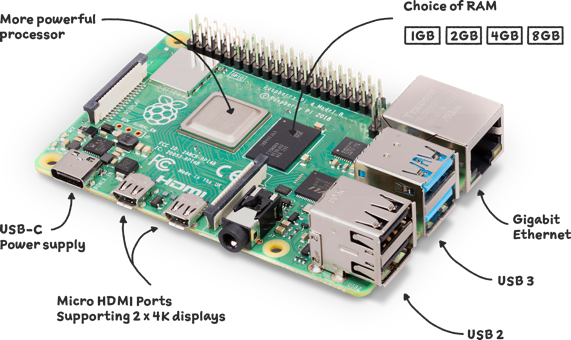
\includegraphics[scale=0.5]{figs/raspberry-pi-4.png}
	\end{center}
	\caption{Raspberry PI 4.} 
\end{figure}

Do ponto de vista de \textit{software}, os Raspberry PI possuem compatibilidade com uma série de \ac{SO} Linux o que 
faz destes componentes também uma opção interessante para a prototipagem de programas mais completos e que vão rodar 
sobre o ambiente de um \ac{SO}.

Apesar da Raspbery disponibilizar em seu site um \ac{SO} específico para uso nesta placa, capaz de extrair melhor 
desenpenho da mesma; no contexto do corrente trabalho o \ac{SO} utilizado foi a atual versão \ac{LTS} do Ubunto Server (22.04),
que por ser uma das versões mais utilizadas mundialmente em servidores garante que todos os códigos utilizados aqui podem 
ser portabilizados para servidores padrão, estejam eles em nuvem ou não. O passo a passo desta instalação pode ser 
encontrado em na página do fabricante. \cite{ubunto-inst}

\section{Mosquitto\textregistered~ Broker}

Desenvolvido pela Eclipse Foudation\textregistered~ o \textit{Broker} Eclipse Mosquitto, ou somente Mosquitto, é uma 
implementação de um \textit{Broker} \ac{MQTT} com interface de simples aprendimento, tanto para instalações locais,
quanto para aquelas feitas de forma remota. Além disso, o Mosquitto é conhecido por ser um programa que requer para 
seu funcionamento poucos recursos seja no âmbito do processamento ou no âmbito do espaço em memória.

Embora muito simples, o \textit{Broker} Mosquitto possui uma série de funções importantes que vão desde segurança via 
certificados x509 até a implementação do modo Bridge: Um modo de funcionamento onde as mensagens publicadas em um 
\textit{Broker} são repetidas em um ou mais espelhos, sendo o contrário também possível todas estas possíveis configurações
podem ser consultadas na documentação dos arquivos ".conf". \cite{mosq-doc}
 


% ----------------------------------------------------------
% Proposta de pesquisa
% ----------------------------------------------------------
\chapter[Proposta]{Proposta}

O principal objetivo deste trabalho é a construção de um framework modular para acesso a diferentes tipos de máquinário
utilizando um componente de baixo custo, no caso o ESP32, via comunicação \ac{MQTT}, para isso foram desenvolvidas algumas 
bibliotecas modulares que podem ser utilizadas para controlar três funções vitais do microcontrolador, de forma a 
tranformá-lo em um componente capaz de funcionar como um intermediário na comunicação do maquinário com a rede em nuvem; 
sendo, neste trabalho, a proposta dividir todo o código em três bibliotecas principais:

\section{ESP-Wifi}

Responsável por gerenciar o acesso dos ESP32 na rede Wifi, importante pois facilita o acesso a rede wifi utilizada 
gerenciando internamente o modelo de acesso que a depender do local e do tipo do experimento mudava de \ac{WPA2-PSK}
para \ac{WPA2-ENT}, vale ressaltar que entre os vários protocolos utilizados no \ac{WPA2-ENT} preferia-se sempre o uso do 
\ac{PEAP-MSCHAPv2}. A \autoref{fig:wifi} apresenta uma representação do sistema de heranças utilizado na biblioteca onde
temos, a partir da classe \textit{Wifi Event Handler} que implementa os métodos para o envio e recebimento de dados,
duas classes derivadas (\textit{WPA2 PSK} e \textit{WPA2 ENT}) com os métodos responsáveis pelo processo de autenticação,
variando para cada protocolo.

\begin{figure}[htb]
    \begin{center}
	    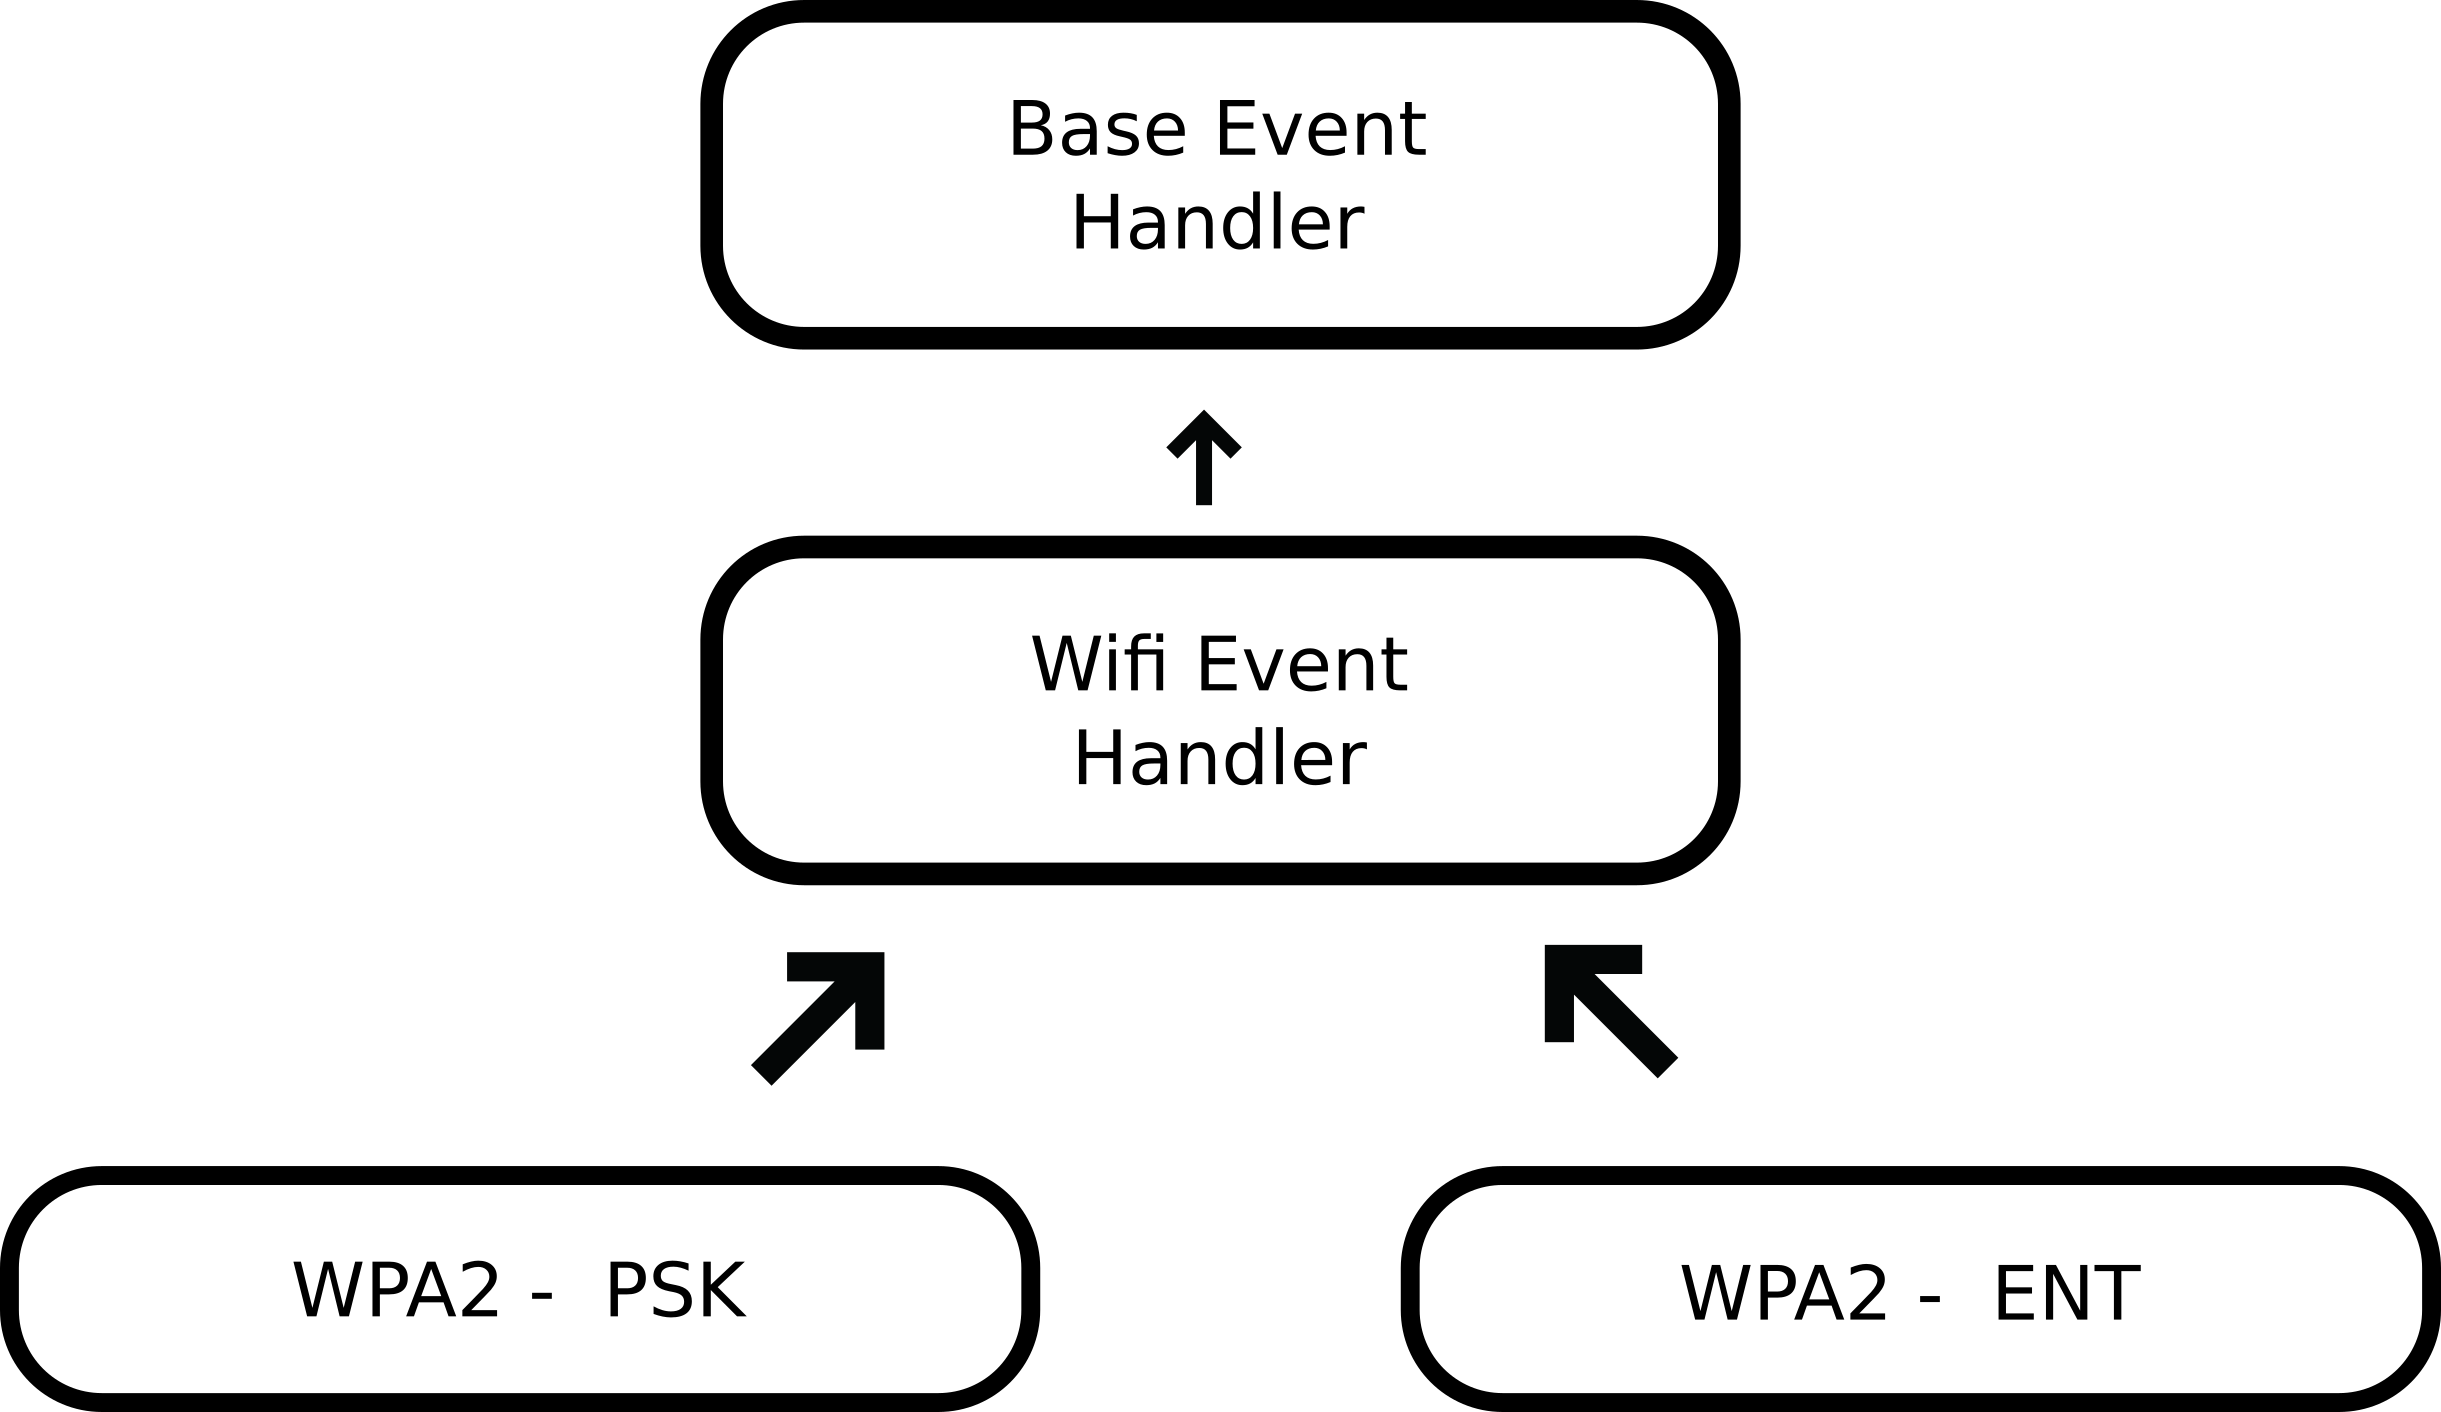
\includegraphics[scale=0.5]{figs/wifi-dia.png}
	\end{center}
	\caption{\label{fig:wifi} Diagrama de herança das classes da biblioteca wifi.} 
\end{figure}

\section{ESP-MQTT}

Responsável por controlar a comunicação \ac{MQTT} como um todo. A maneira utilizada para implementar o protocolo se 
baseia no sistema de eventos, onde cada evento está relacionado com uma etapa do estabelecimento da comunicação, 
porém as funções chamadas em cada um das etapas são métodos de uma classe que representa a conexão, de forma que 
a implementação da biblioteca em projetos futuros fique bem simples, se limitando a pouco mais do que instanciar o 
objeto e chamar o método \textit{PostData}. A \autoref{fig:mqtt} apresenta o modelo utilizado, apresentando os métodos
padrão para o estabelecimento da conexão \ac{MQTT} (destacados em \textit{MQTT Standard Events}) e os \textit{Hi-Level Events}
que simplificam o processo de envio e serão os únicos utilizados doravante.

\begin{figure}[htb]
    \begin{center}
	    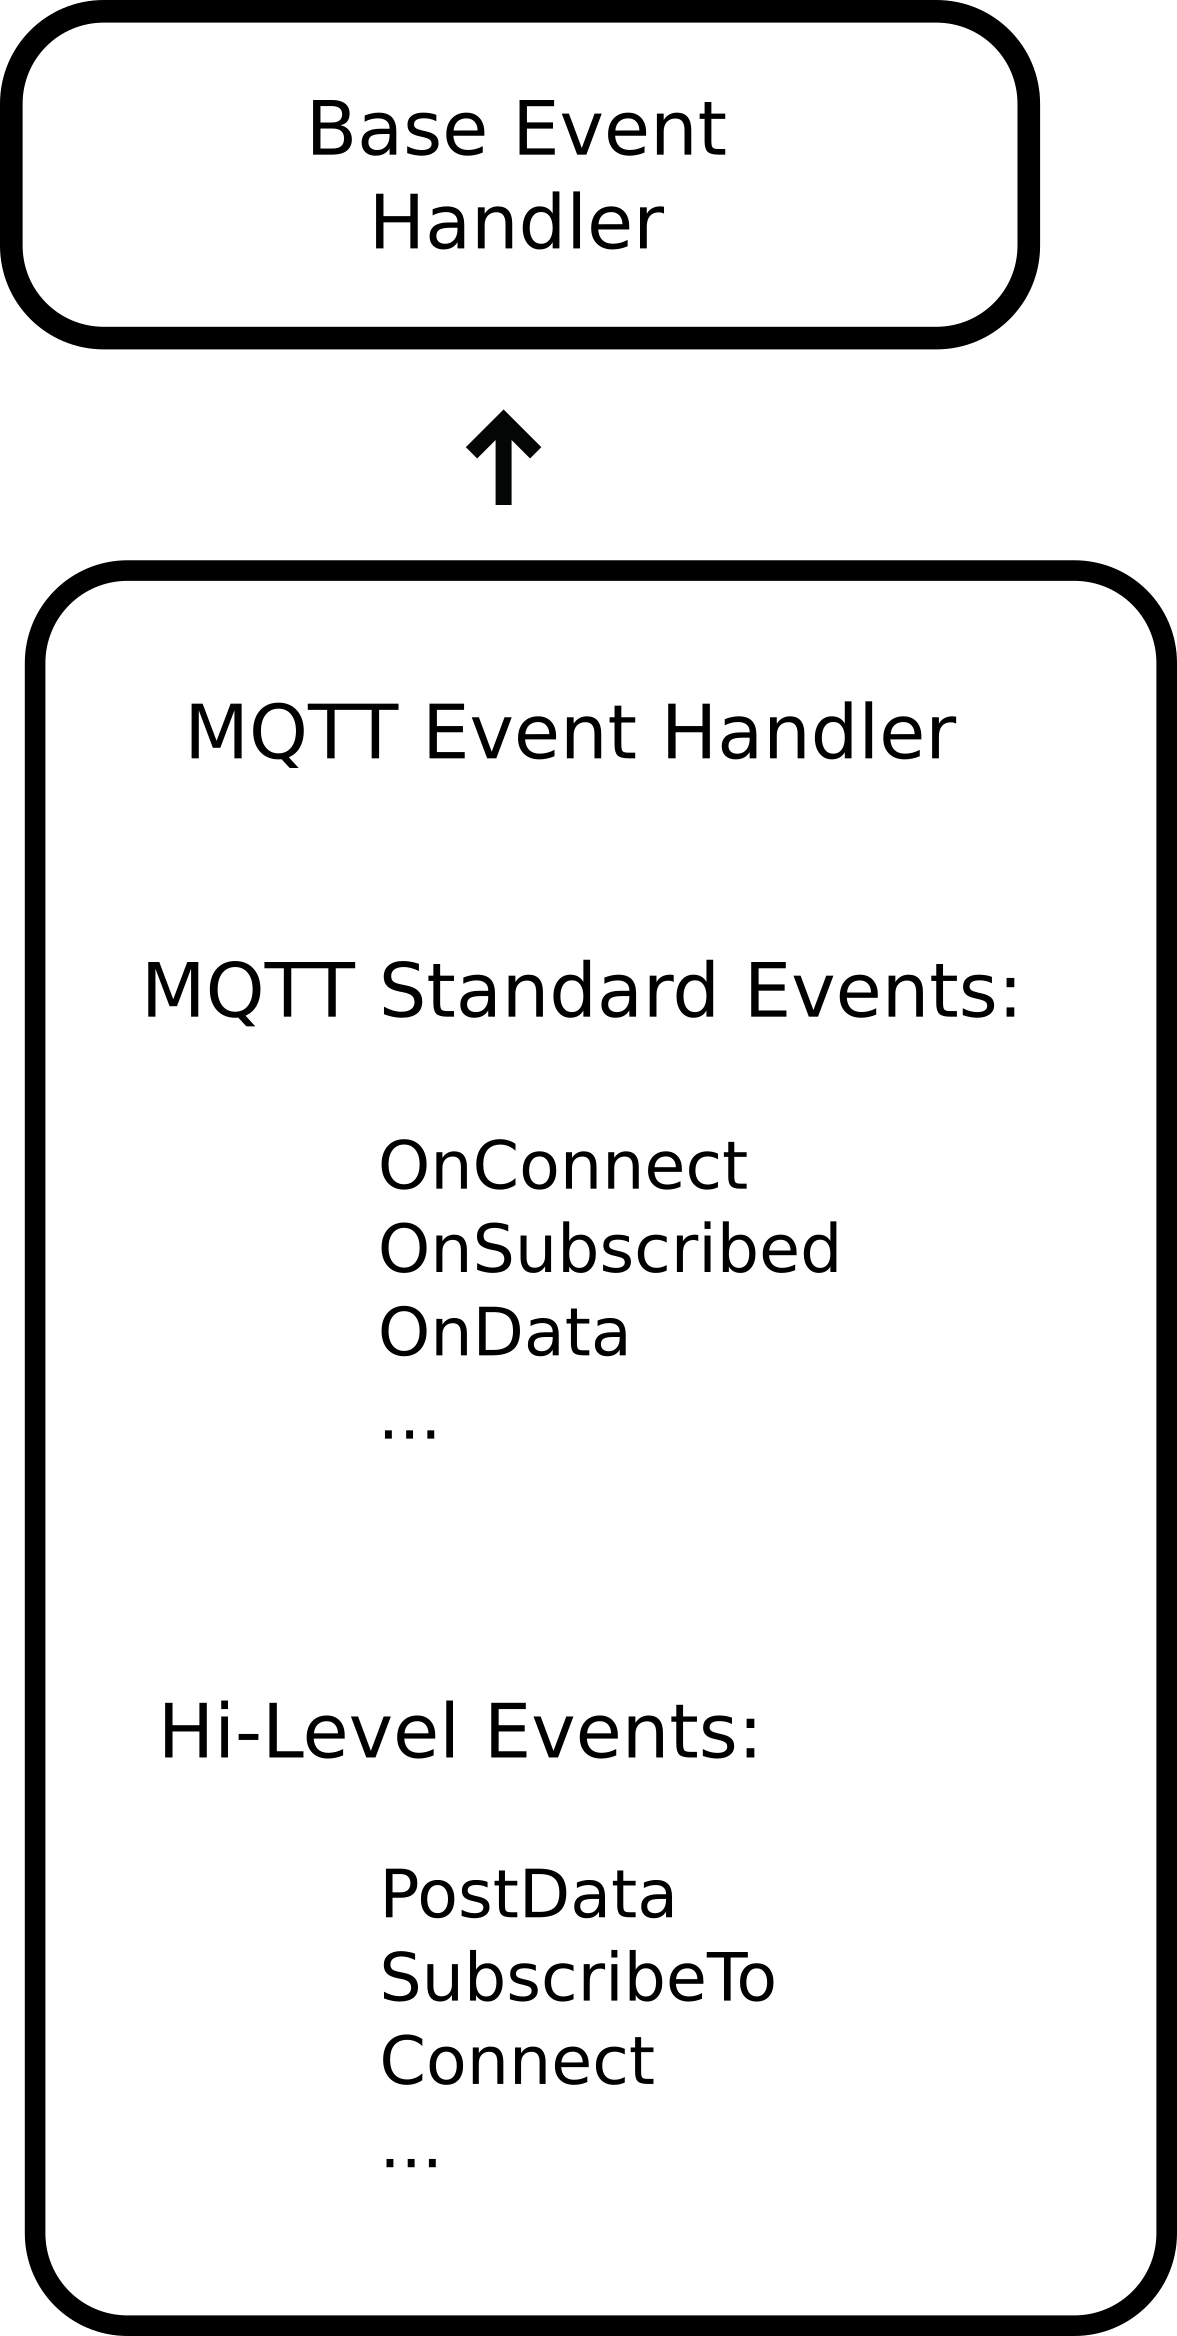
\includegraphics[scale=0.5]{figs/mqtt-dia.png}
	\end{center}
	\caption{\label{fig:mqtt} Diagrama esquemático da classe MQTT.} 
\end{figure}


\section{ESP-Serial}

Responsável por controlar a comunicação serial via \ac{UART} com diversos componentes. Do ponto de vista da arquitetura
ela segue os mesmos conceitos utilizados pela biblioteca responsável pelo \ac{MQTT} com as diferenças sendo basicamente
internas nas partes responsáveis pela instalação dos drivers para utilização dos pinos dos componentes. A \autoref{fig:serial}
apresenta a estrutura da classe desenvolvida para comunicação serial. 

\begin{figure}[htb]
    \begin{center}
	    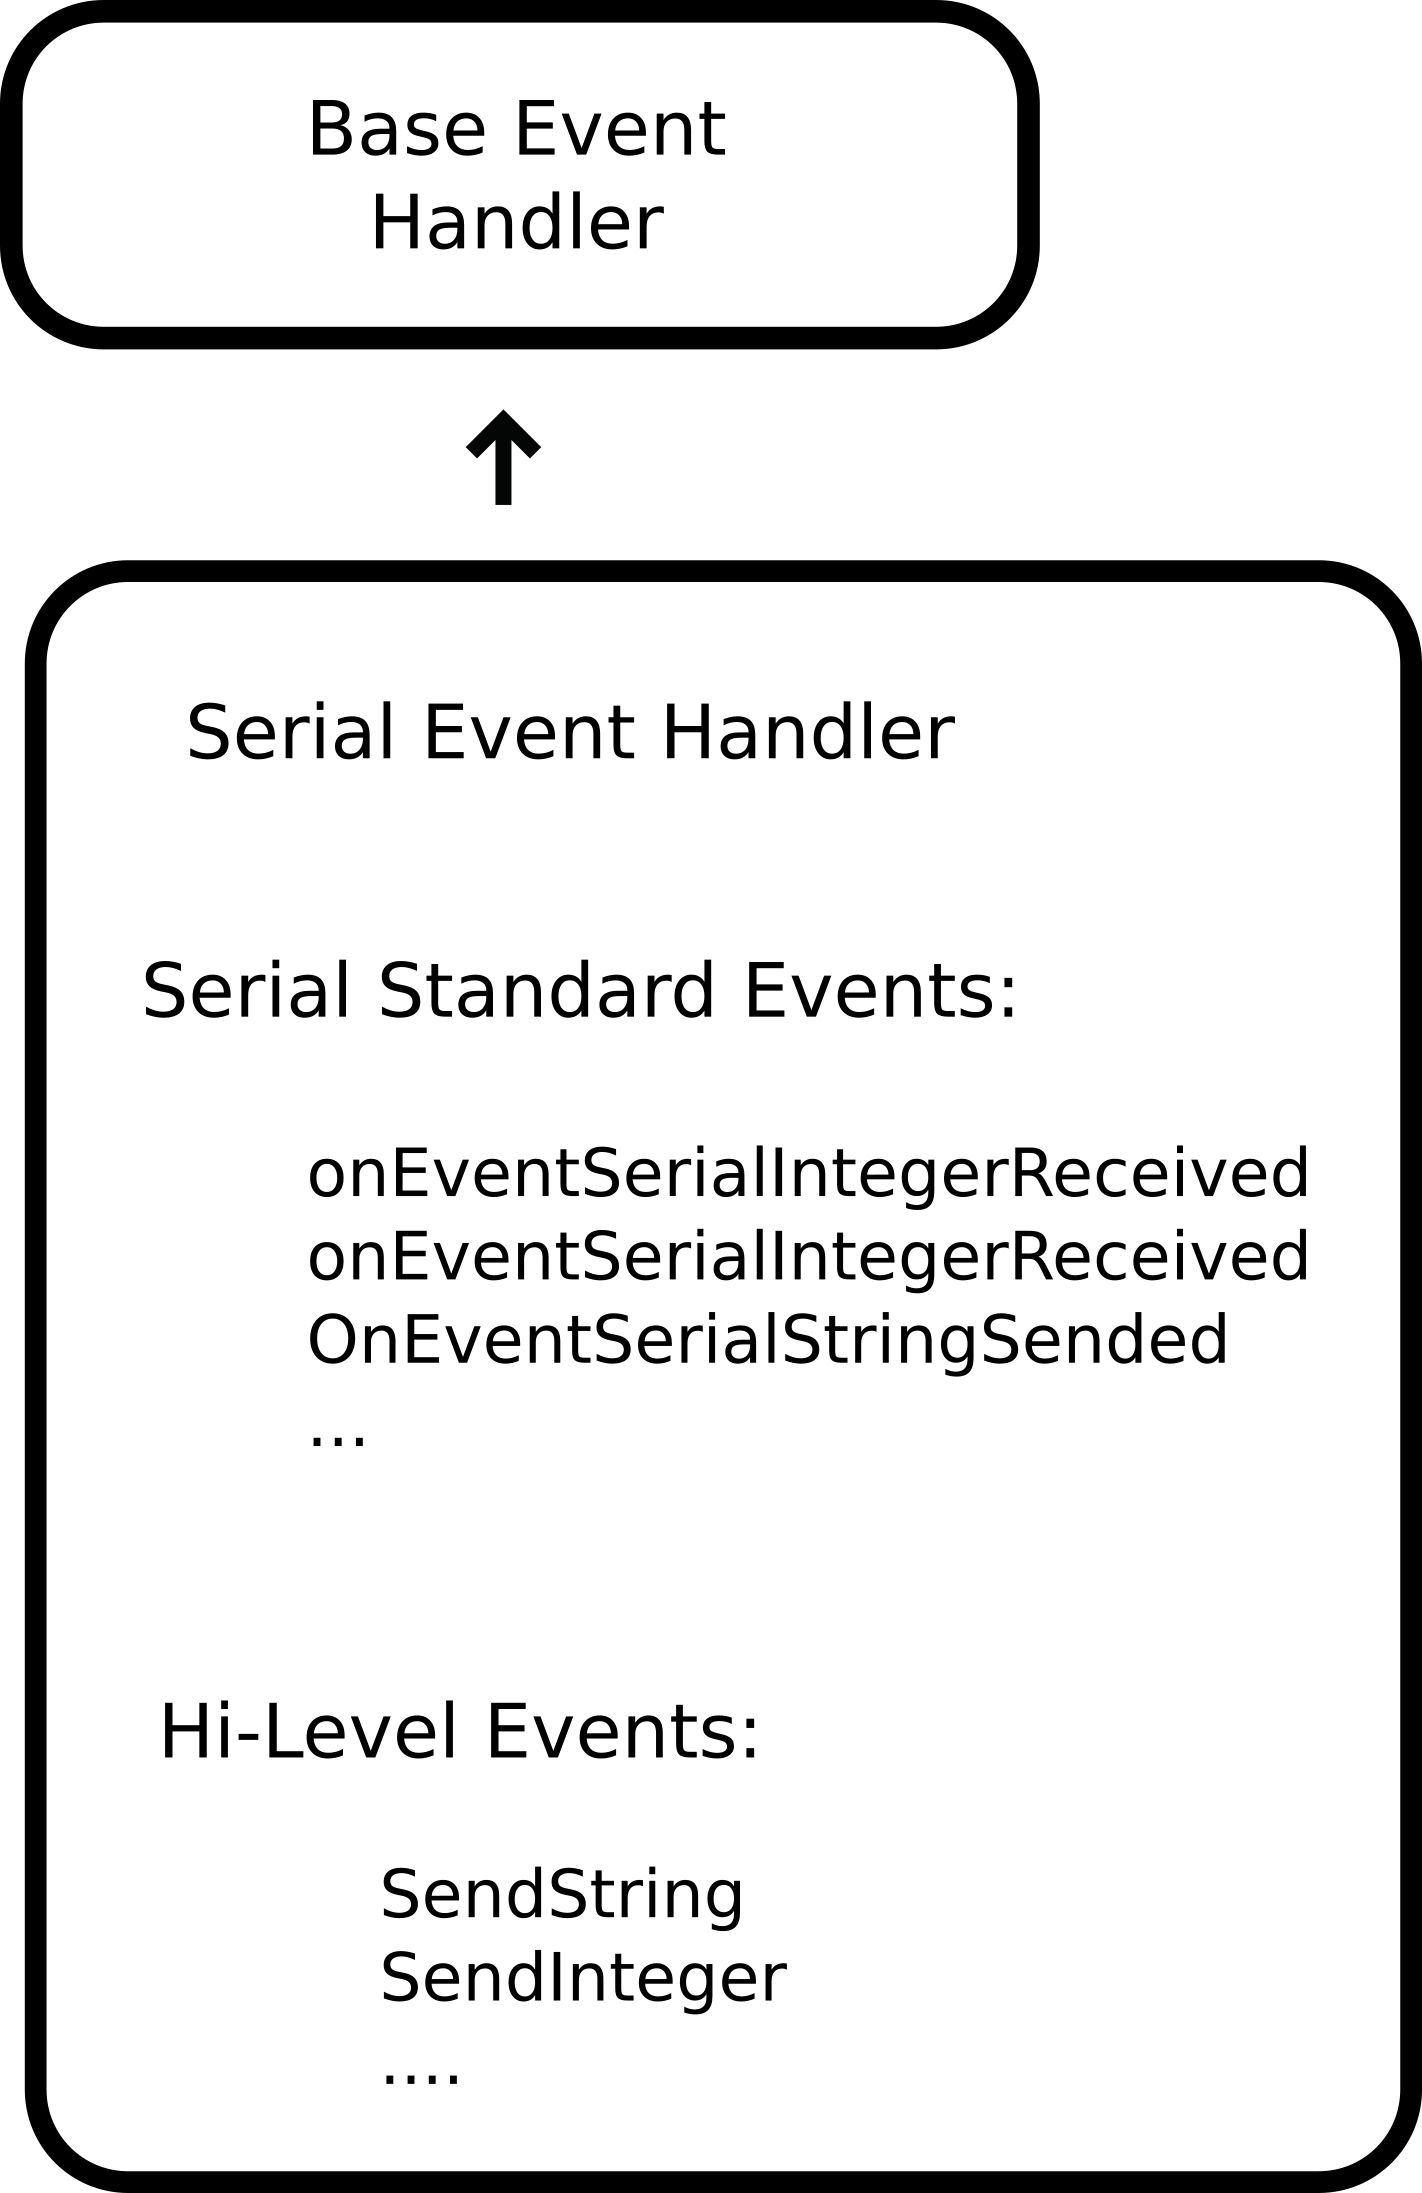
\includegraphics[scale=0.5]{figs/serial-dia.png}
	\end{center}
	\caption{\label{fig:serial} Diagrama esquemático da classe serial.} 
\end{figure}

\newpage
Uma colocação importante é a de que estas bibliotecas seguem o modelo de desenvolvimento dos componentes do \ac{ESP-IDF}
\footnote{O Framework de desenvolvimento dos ESP32 possui uma documentação bastante robusta e pode ser encontrada em 
\url{https://docs.espressif.com/projects/esp-idf/en/latest/esp32/index.html}\cite{esp-idf-docs}}
de forma que eles devem ser independentes e podem ser facilmente incorporados a códigos de terceiros
\footnote{Na documentação das bibliotecas no repositório existe um passo a passo de como essa importação pode feita 
utilizado somente um comando dos \textit{submodules} do GIT: \url{https://github.com/MAPL-UFU/IndustrialAutomationMQTT}},
 mas que quando utilizados em conjunto apresentam ganhos, pois o fato de utilizarem a mesma classe mãe (\textit{Base Event Handler}) garante que eles utilizem
 somente um \textit{loop} de eventos e, portanto, menos recursos em memória já que na implemetação do \ac{ESP-IDF} todos 
 os \textit{loops} de eventos possuem no mínimo uma \textit{task} em memória associada. 

Por fim, um segundo objetivo deste trabalho é propor um modelo de comunicação que possua meios para garantir a comunicação
local, diretamente via \ac{MQTT}, mesmo no caso de falhas dos servidores em nuvem, para isso foi utilizado localmente
o \textit{Broker} Mosquitto\textregistered~ em modo \textit{Bridge}, em que, como foi mencionado na fundamentação teórica,
é possível replicar mensagens de tópicos específicos em \textit{Brokers} distintos, os códigos de configuração utilizados 
estão no \autoref{ape:moss}.





% ----------------------------------------------------------
% Experimentos e avaliação dos resultados
% ----------------------------------------------------------

\newpage
\chapter[Experimentos e Análise dos Resultados]{Experimentos e Análise dos Resultados}
\label{experimentos}

Como já especificado em capítulos anteriores, este trabalho de dispõe a apresentar um Framework de 
 controle para sistemas discretos de forma a utilizar os principais ganhos do protocolo \ac{MQTT} para propor soluções mais 
 simples do que as amplamente utilizadas em processos industriais para problemas como gerenciamento da rede, custo dos 
 equipamentos utilizados e entre outros. Neste sentido, o principal teste realizado foram a realização de duas provas de
 conceito simulando sistemas amplamente presentes no âmbito industrial para se observar o comportamento do modelo 
 proposto, além disso, a partir das simulações foram encontradas algumas questões para as quais foram propostos testes 
 especiais assim como descrito a seguir.

\section{Método para a Avaliação}
\label{metodo}

O método utilizado para avaliar a funcionalidade do sistema proposto foi a implementação direta de duas provas de 
conceitos utilizando o material do \ac{LEM}, isto é, a montagem de um circuito eletro-pneumático 
(primeiramente, mas posteriormente foram feitos testes também com sistemas eletro-hidráulicos) para controle de um ou mais 
cilindros utilizando o sistema \ac{MQTT} para promover a comunicação em Edge e em nuvem.

\section{Experimentos}

\subsection{Experimento 1 — Controle de 1 cilindro}

\begin{figure}[htb]
    \begin{center}
	    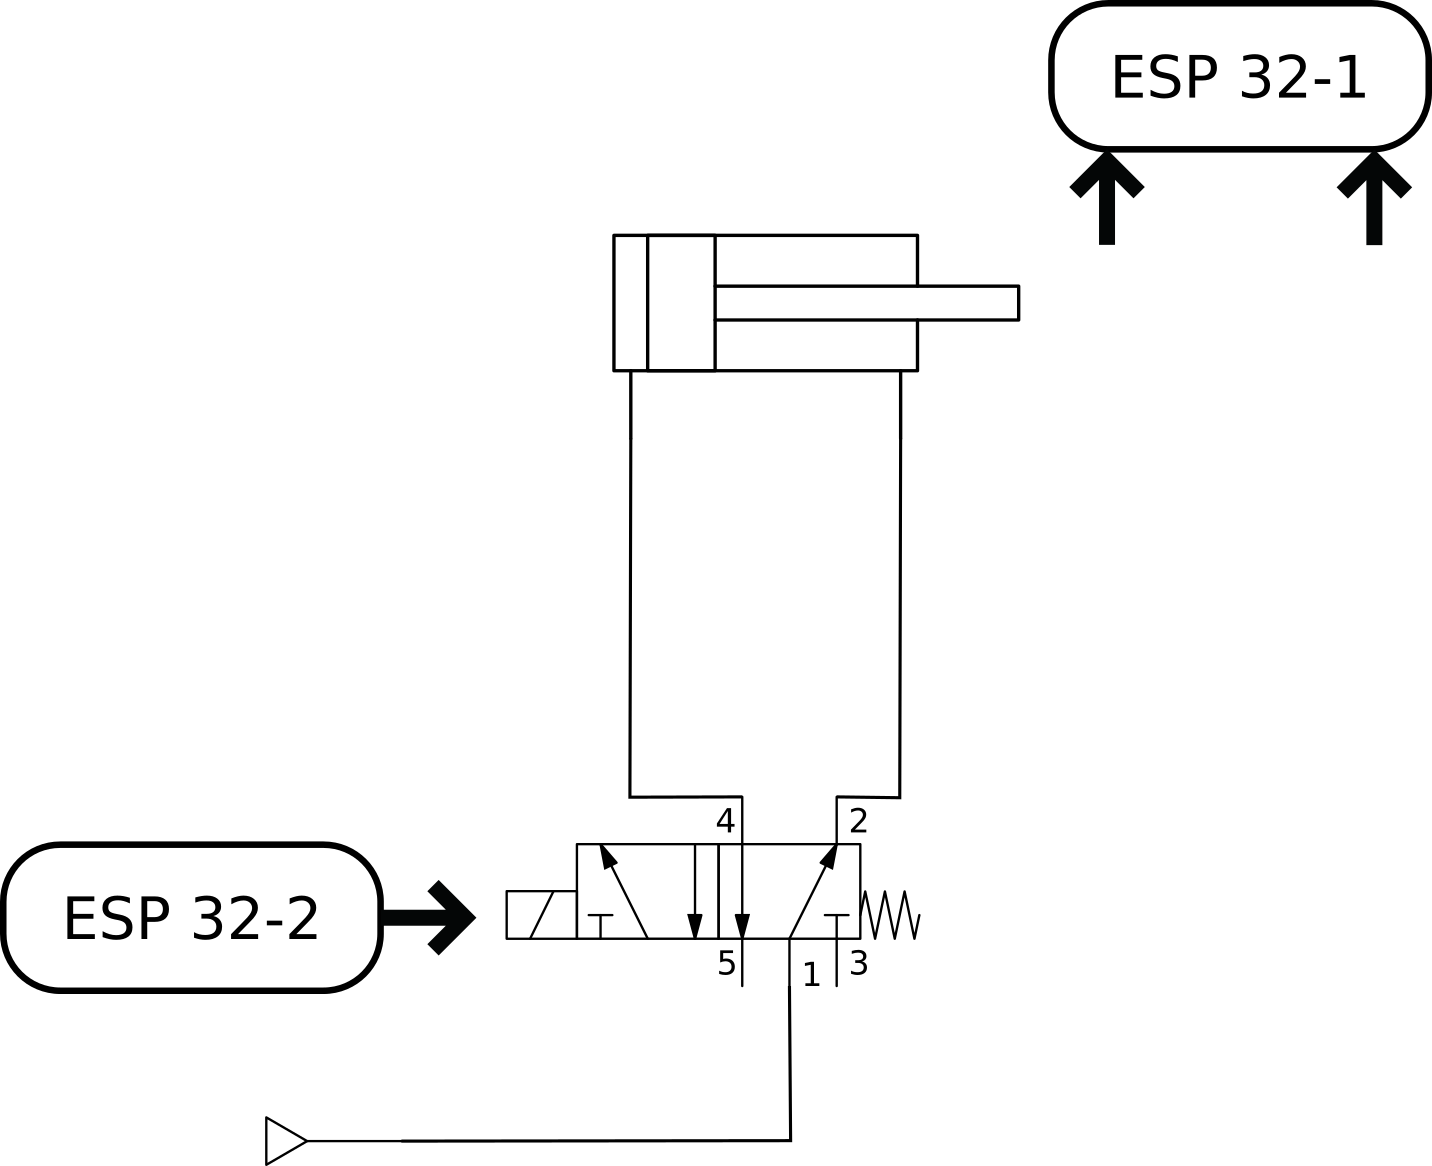
\includegraphics[scale=0.5]{figs/diag_exp1.png}
	\end{center}
	\caption{\label{fig:exp1} Diagrama do primeiro experimento realizado.} 
\end{figure}

O primeiro experimento realizado se dispunha a realizar o controle de apenas um cilindro pneumático de forma que dois
ESP32 foram utilizados no sistema \ac{MQTT} para promover a comunicação, um microcontrolador era responsável por monitorar 
os sensores e disponibilizar seu estado em rede, assim sendo caracterizado como um publicador; enquanto o outro 
microcontrolador era responsável por controlar o estado do cilindro utilizando as informações disponibilizadas pelos 
sensores assim, assim sendo caracterizado como um subscritor. Na \autoref{fig:exp1} existe um diagrama da montagem 
realizada. Neste Exemplo, foram utilizados tanto a implementação local do \textit{Broker Eclipse Mosquitto\textregistered~}quanto 
o disponibilizado pela AWS\textregistered~, AWS Iot Core. Vale ressaltar que no caso do \textit{Broker} via AWS foi necessário a 
implementação de Segurança \ac{TLS} e dos Certificados x.509 gerados diretamente na plataforma para a utilização do \textit{Broker}
\footnote{O caminho para conexão de novos dispositivos pode ser facilmente encontrado no caminho: 
AWS Iot > Connect > Connect one device}, 
desta forma, seguindo o passo a passo descrito na própria plataforma foram geradas a Política e o Certificado de cada ESP
sendo de forma que cada um possui um \textit{Endpoint} dedicado para conexão, ambos capazes de ler e publicar no tópico "lem/valve"
a \autoref{fig:cert1} mostra a estrutura característica utilizada para cadastro dos itens na AWS. No apendice \autoref{ape:exp1} 
estão disponibilizados os trechos do código responsáveis especificadamente pela transmissão dos dados via \ac{MQTT}, porém
caso queira consultar os códigos completos de cada aplicação (experimento um e dois, ou ainda das bibliotecas que contituem o \textit{Framework})
eles estão disponíveis e documentados repositório no Github\textregistered~ do Laboratório de Planejamento Automático de Manufatura \footnote{
    Disponível em: \url{https://github.com/MAPL-UFU/IndustrialAutomationMQTT}}.

\begin{figure}[htb]
    \begin{center}
	    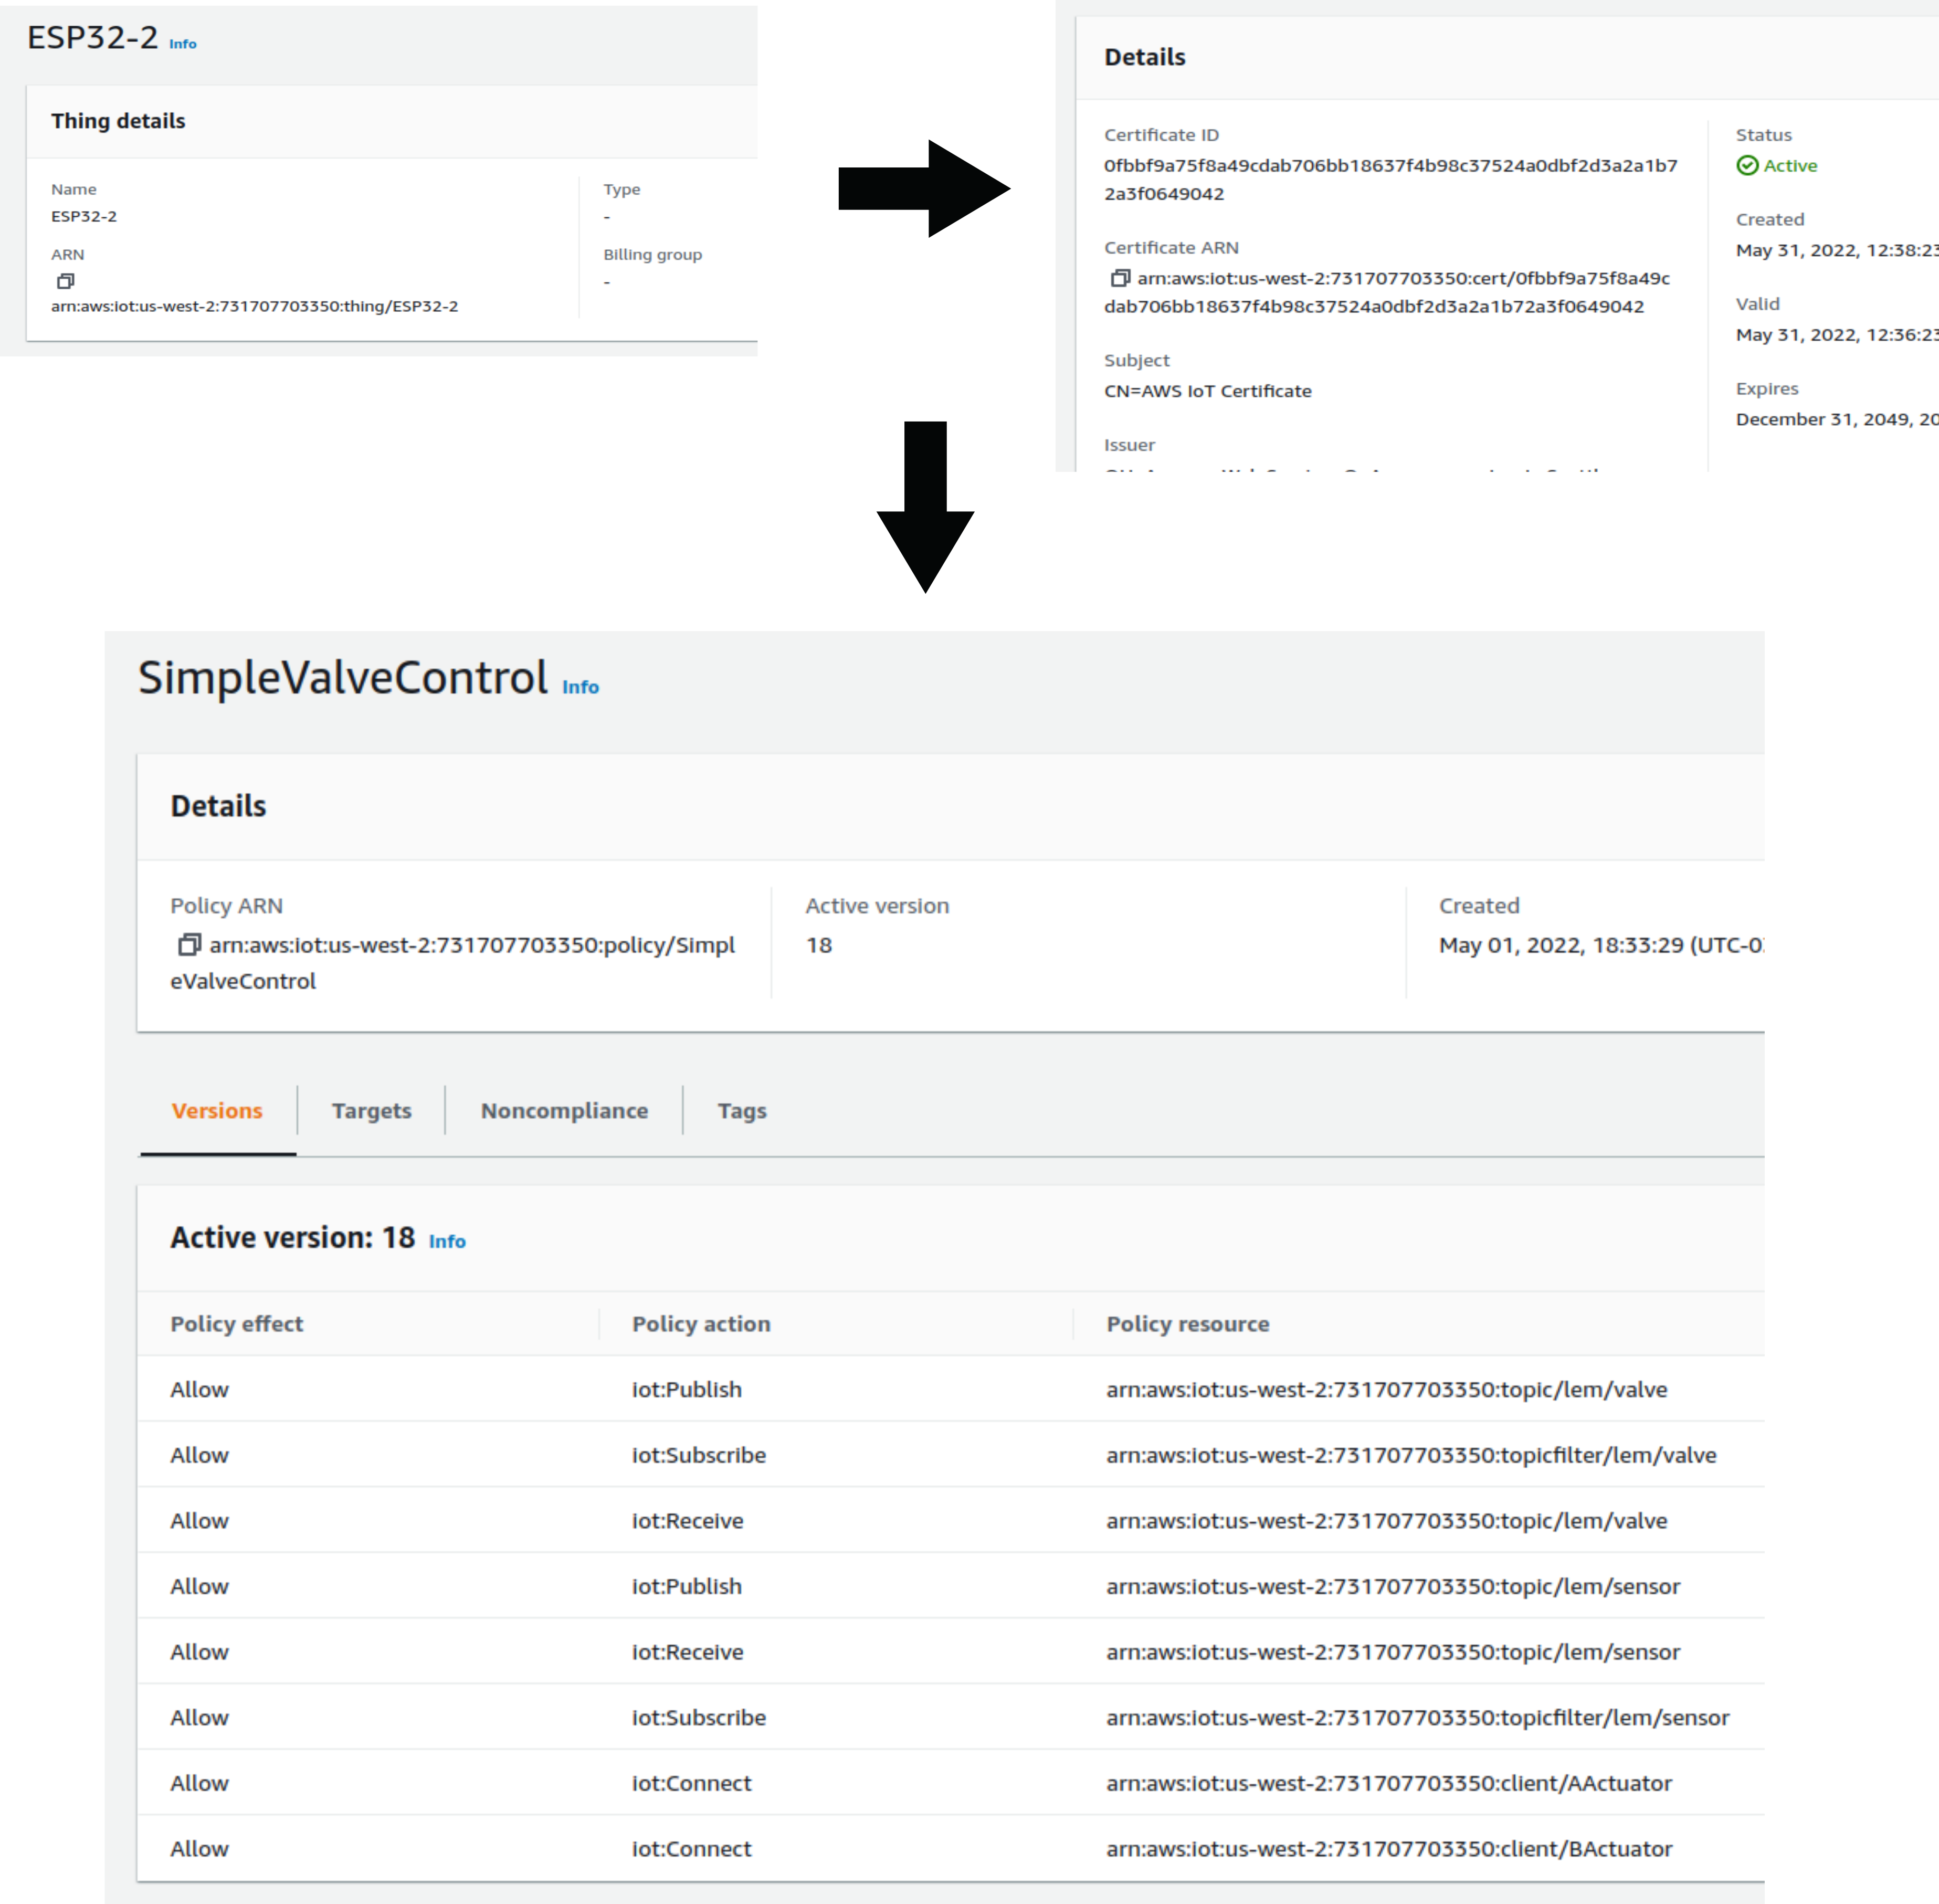
\includegraphics[scale=0.5]{figs/cert_flow.png}
	\end{center}
	\caption{\label{fig:cert1} Estrutura de permissões .} 
\end{figure}


\subsection{Experimento 2 — Controle de 2 cilindros}


\begin{figure}[htb]
    \begin{center}
	    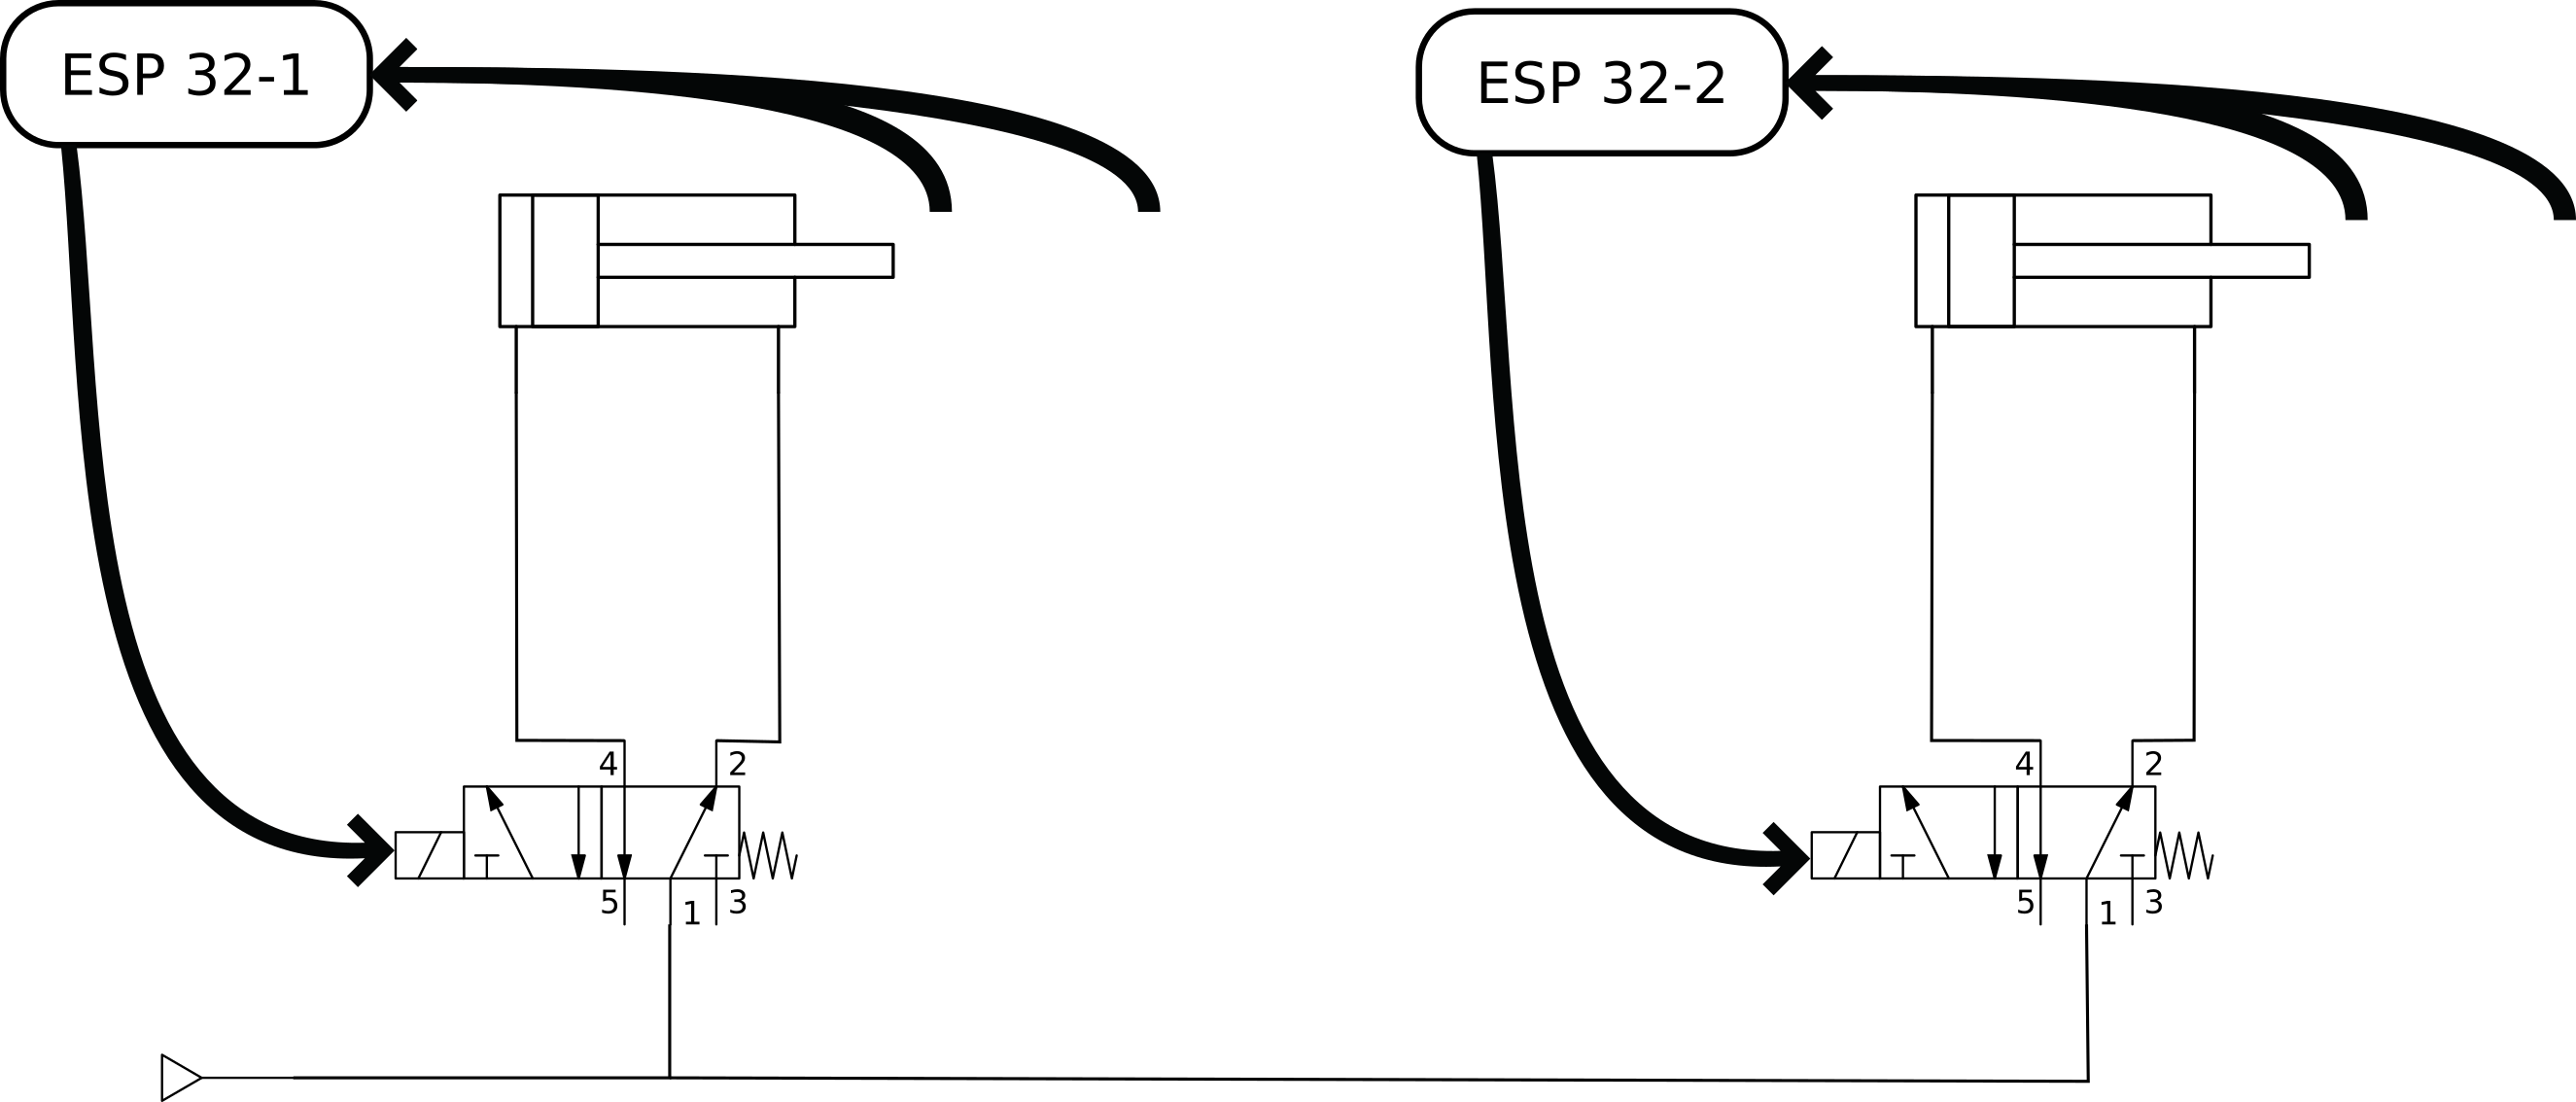
\includegraphics[scale=0.5]{figs/diag_exp2.png}
	\end{center}
	\caption{\label{fig:exp2} Diagrama do segundo experimento realizado.} 
\end{figure}

Já no segundo Experimento, foi utilizada uma montagem onde cada Esp-32 era responsável por um cilindro, isto é, 
controlando tanto suas entradas como suas saídas, assim cada cilindro é, ao mesmo tempo, um publicador e um subscritor.
Na \autoref{fig:exp2} existe um diagrama da montagem realizada. Neste experimento não foram utilizados os recursos da AWS,
em vez disso, agora que já tínhamos testado a comunicação
pela rede deles, neste segundo momento optou-se pelos serviços gratuitos disponibilizados pelo site shiftr.io já que o foco 
não era os elementos de segurança da rede em si, implementação do \ac{SSL} ou geração das permisões. A essa altura o
objetivo era a inclusão de um terceiro elemento na rede responsável por duas coisas: funcionar como um servidor de lógica,
ou seja, um item externo que relaciona as saídas dos sensores às entradas dos atuadores e também de um servidor \ac{MQTT} local
que fosse capaz de se comunicar de forma \textit{full-duplex} com o servidor em nuvem, como apresentado na 
\autoref{fig:conn}, permitindo que o sistema fosse acessado 
remotamente, mas sem deixá-lo totalmente dependente da nuvem, de forma que o mesmo continua funcionando em casos em que 
a comunicação entre a rede local e a Internet é perdida. O arquivo de configuração do \textit{Broker} local pode ser consultado
no \autoref{ape:moss}.

\begin{figure}[htb]
    \begin{center}
	    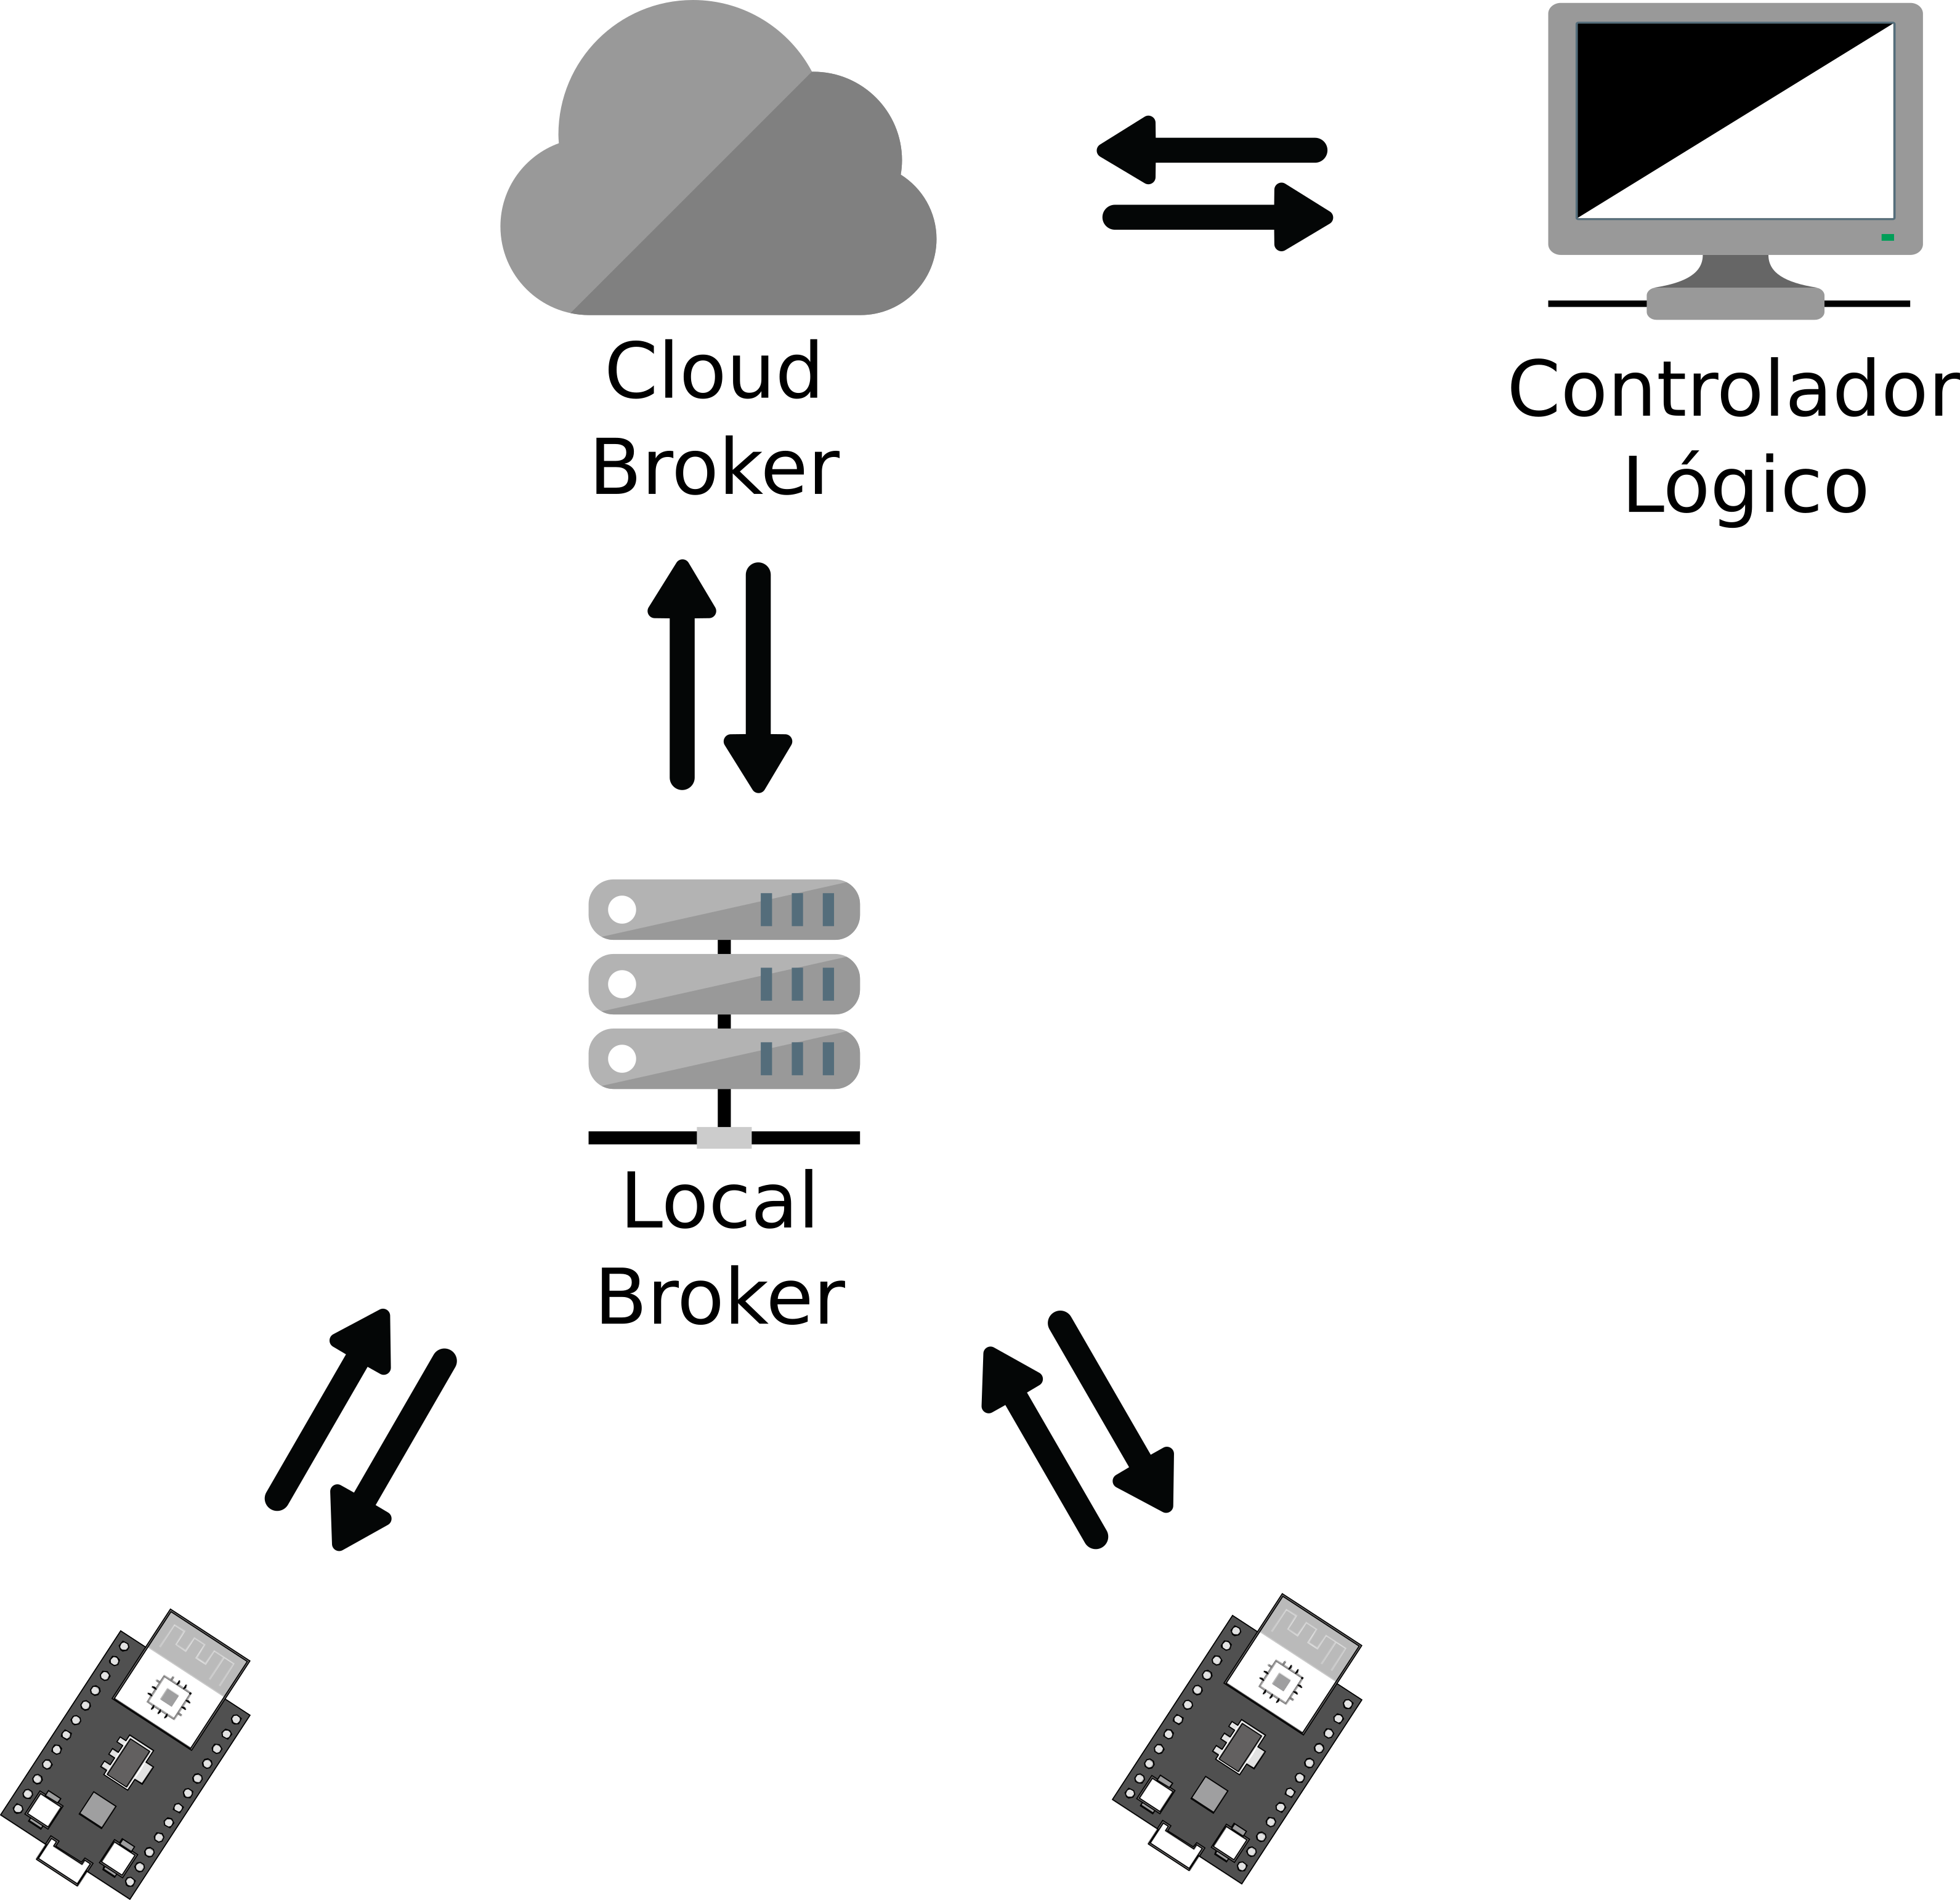
\includegraphics[width=300pt]{figs/diag_conn.png}
	\end{center}
	\caption{\label{fig:conn} Diagrama da comunicação entre o Broker local e em nuvem.} 
\end{figure}


Como elemento extra foi utilizado a título de exemplo um Raspberry Pi 4; no qual, beneficiando-se do isolamento de processos 
característico de sistemas operacionais, era possível a implementação simultânea do broker \ac{MQTT} Mosquitto e de um \textit{script 
Python} para controle do sistema. Assim, para a parte de lógica foi utilizada a biblioteca própria para comunicação com 
servers \ac{MQTT} Paho, pois dada a praticidade dos \textit{scripts Python} ficava bem simples a aplicação da lógica e a implementação 
de possíveis modificações já com o sistema funcionando, o código \textit{Python} utilizado se encontra no \autoref{ape:py}. Por fim, na implementação do \textit{Broker Mosquitto} foi utilizada uma 
função chamada \ac{MQTT} Bridge\cite{mosq-doc} configurada de forma que todos os tópicos utilizados no sistema estão sendo 
replicados nos dois Brokers assim garantindo que uma queda na Internet não quebrará todo o sistema, além de possibilitar
que sejam colocados lógicas de segurança em Edge para casos onde uma parada abrupta geraria sérios problemas.

\section{Avaliação dos Resultados}
\label{avaliacao}

\begin{figure}[htb]
    \begin{center}
        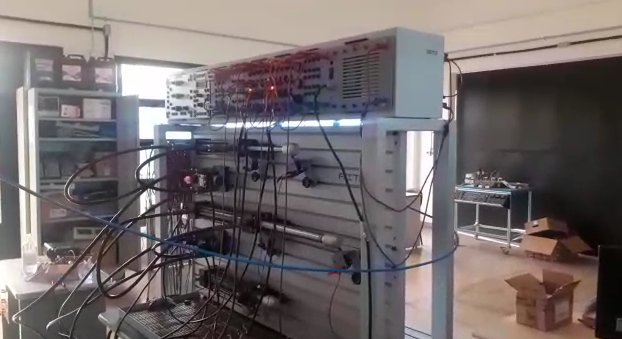
\includegraphics[scale=0.5]{figs/exp_h.png}
    \end{center}
    \caption{\label{fig:exp_m1} Montagem realizada na bancada hidráulica.} 
\end{figure}

\begin{figure}[htb]
    \begin{center}
	    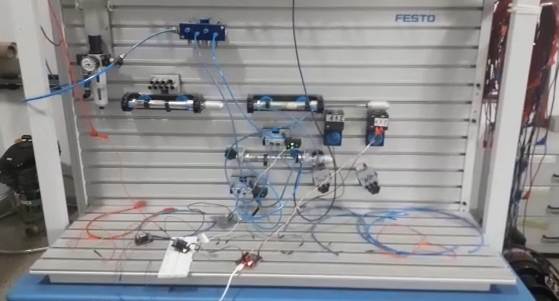
\includegraphics[scale=0.5]{figs/exp_p.png}
	\end{center}
	\caption{\label{fig:exp_m2} Montagem realizada na bancada pneumática.} 
\end{figure}


Após a implementação em bancada do sistema, o que pode ser visto na \autoref{fig:exp_m1} e na \autoref{fig:exp_m1},
obteve-se sucesso com a comunicação e com o funcionamento do sistema como um todo,
em ambas as montagens. Porém, foram encontradas alguns problemas na transmissão das informações que, embora não sejam
capazes de inviabilizar o sistema conforme os objetivos preestabelecidos para o estudo atual, são possíveis objetos de 
estudo para trabalhos posteriores, sendo eles principalmente o aumento da lentidão na troca de informações dependendo da 
Nuvem utilizada, o que não era perceptível no primeiro teste, na bancada hidráulica; mas acabou ficando evidente nos testes
utilizando o circuito pneumático e a inclusão de ruído proveniente dos sensores utilizados na montagem
também a depender do atuador e dos sensores de contato utilizados. Vale ressaltar, ainda, que a velocidade na transmissão
de mensagens sofria grandes variações de acordo com o \textit{Broker} utilizado, sendo praticamente instantânea em aplicações com
\textit{Broker} local, tendo pequeno atraso quando instanciado utilizando a nuvem AWS, e maior atraso quando utilizada a
nuvem disponibilizada pelo \textit{shiftr.io}~\textregistered.

% ---
% Finaliza a parte no bookmark do PDF, para que se inicie o bookmark na raiz
% ---
\bookmarksetup{startatroot}% 
% ---

% ---
% Conclusão
% ---
\chapter[Conclusão]{Conclusão}
Faça uma breve introdução para o capítulo. Observe os objetivos geral e específicos do trabalho no capítulo de introdução e coloque aqui um comentário sobre como o desenvolvimento ajudou a chegar a cada um desses objetivos, ou seja, como a pesquisa permitiu concluir que cada um dos objetivos foi atingido.

\section{Principais Contribuições}
Nessa seção destaque ainda mais as suas contribuições, mostrando que sua hipótese foi validada pelos experimentos executados. 

\section{Trabalhos Futuros}
Destaque nessa seção o que pode ser melhorado no método proposto para resolver as possíveis falhas que você identificou e descreveu na seção \ref{avaliacao}. Indique quais outros projetos podem ser gerados a partir do seu trabalho.

\section{Contribuições em Produção Bibliográfica}
Liste a produção bibliográfica resultante do seu trabalho.


 

% ----------------------------------------------------------
% ELEMENTOS PÓS-TEXTUAIS
% ----------------------------------------------------------
\postextual

% ----------------------------------------------------------
% Referências bibliográficas
% ----------------------------------------------------------
\bibliography{bib/referencias}


% ----------------------------------------------------------
% Apêndices
% ----------------------------------------------------------
% ---
% Inicia os apêndices
% ---
\begin{apendicesenv}
% Imprime uma página indicando o início dos apêndices
\partapendices
% ----------------------------------------------------------
% Incluir Apêndice
% ----------------------------------------------------------
% ----------------------------------------------------------
% Capitulo com exemplos de comandos inseridos de arquivo externo 
% ----------------------------------------------------------
\chapter[Arquivo de Configuração do Broker]{Arquivo de configuração para utilização do Mosquitto\textregistered~\textit{Broker} em modo \textit{Bridge}}

\label{ape:moss}

\definecolor{darkgreen}{RGB}{0,125,0}

\lstset{ % General setup for the package
    basicstyle=\small,
    numbers=left,
     numberstyle=\tiny,
    frame=tb,
    tabsize=2,
    columns=fixed,
    showstringspaces=false,
    showtabs=false,
    keepspaces
}

\lstinputlisting{ape_codigos_mosquitto/mosquitto.conf}

\chapter[Arquivo de Configuração do Broker]{Arquivo de configuração para utilização do Mosquitto\textregistered~\textit{Broker} em modo \textit{Bridge}}

\label{ape:moss}

\definecolor{darkgreen}{RGB}{0,125,0}

\lstset{ % General setup for the package
    basicstyle=\small,
    numbers=left,
     numberstyle=\tiny,
    frame=tb,
    tabsize=2,
    columns=fixed,
    showstringspaces=false,
    showtabs=false,
    keepspaces
}

\lstinputlisting{ape_codigos_mosquitto/mosquitto.conf}

\chapter[Arquivo de Configuração do Broker]{Arquivo de configuração para utilização do Mosquitto\textregistered~\textit{Broker} em modo \textit{Bridge}}

\label{ape:moss}

\definecolor{darkgreen}{RGB}{0,125,0}

\lstset{ % General setup for the package
    basicstyle=\small,
    numbers=left,
     numberstyle=\tiny,
    frame=tb,
    tabsize=2,
    columns=fixed,
    showstringspaces=false,
    showtabs=false,
    keepspaces
}

\lstinputlisting{ape_codigos_mosquitto/mosquitto.conf}

\chapter[Arquivo de Configuração do Broker]{Arquivo de configuração para utilização do Mosquitto\textregistered~\textit{Broker} em modo \textit{Bridge}}

\label{ape:moss}

\definecolor{darkgreen}{RGB}{0,125,0}

\lstset{ % General setup for the package
    basicstyle=\small,
    numbers=left,
     numberstyle=\tiny,
    frame=tb,
    tabsize=2,
    columns=fixed,
    showstringspaces=false,
    showtabs=false,
    keepspaces
}

\lstinputlisting{ape_codigos_mosquitto/mosquitto.conf}


\end{apendicesenv}
% ---

% ----------------------------------------------------------
% Anexos
% ----------------------------------------------------------
% ---
% Inicia os anexos
% ---
\begin{anexosenv}
    % Imprime uma página indicando o início dos anexos
\partanexos
    % ---
    % Incluir Anexo
    % ---
\chapter[Documentação do Modo Bridge]{Documentação official do modo \textit{Bridge} disponibilizado pelo Mosquitto\textregistered~}

\label{ane:bridge}

\newpage
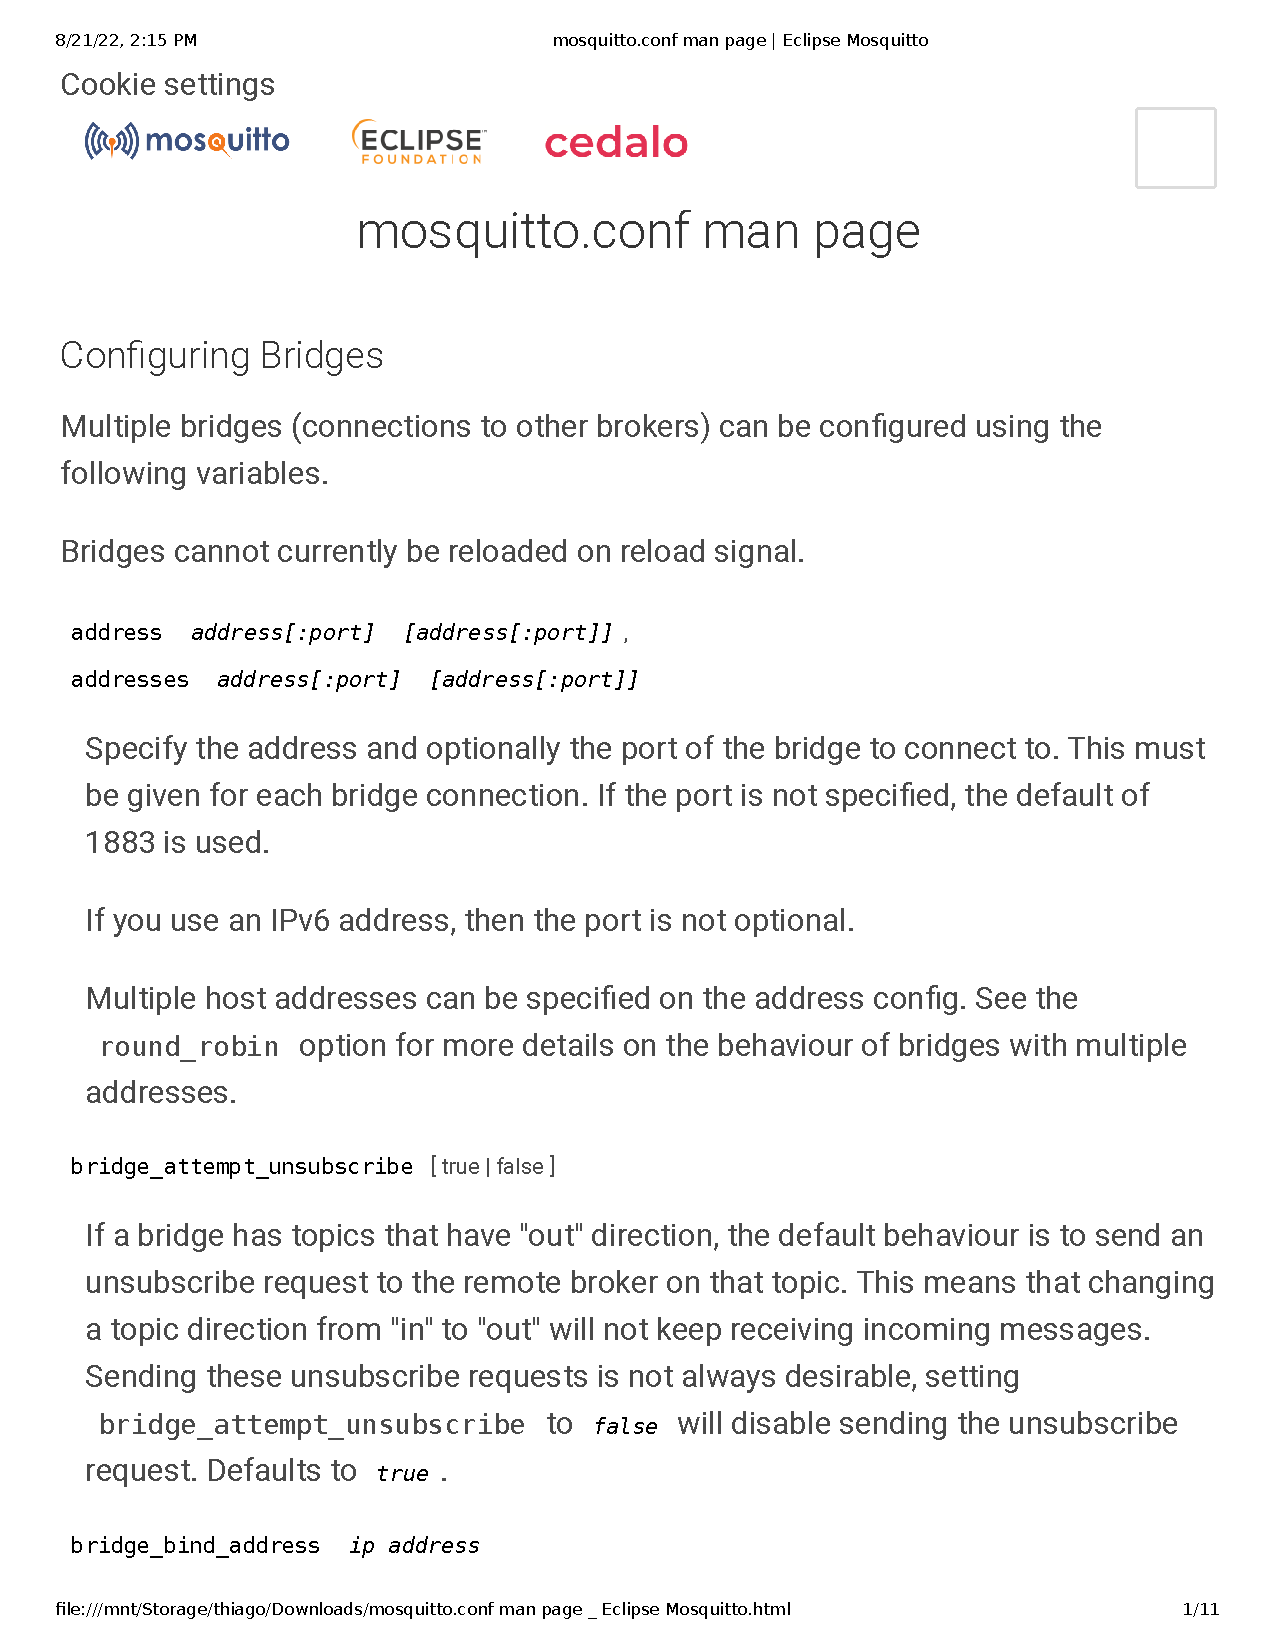
\includepdf[pages=1-11]{ane_mosq_bridge_doc/bridge_conf_man.pdf}
\chapter[Esquema DevKit]{Desenho Esquemático Módulo ESP32-DevKitC-v4}

\label{ane:kit}

\begin{landscape}
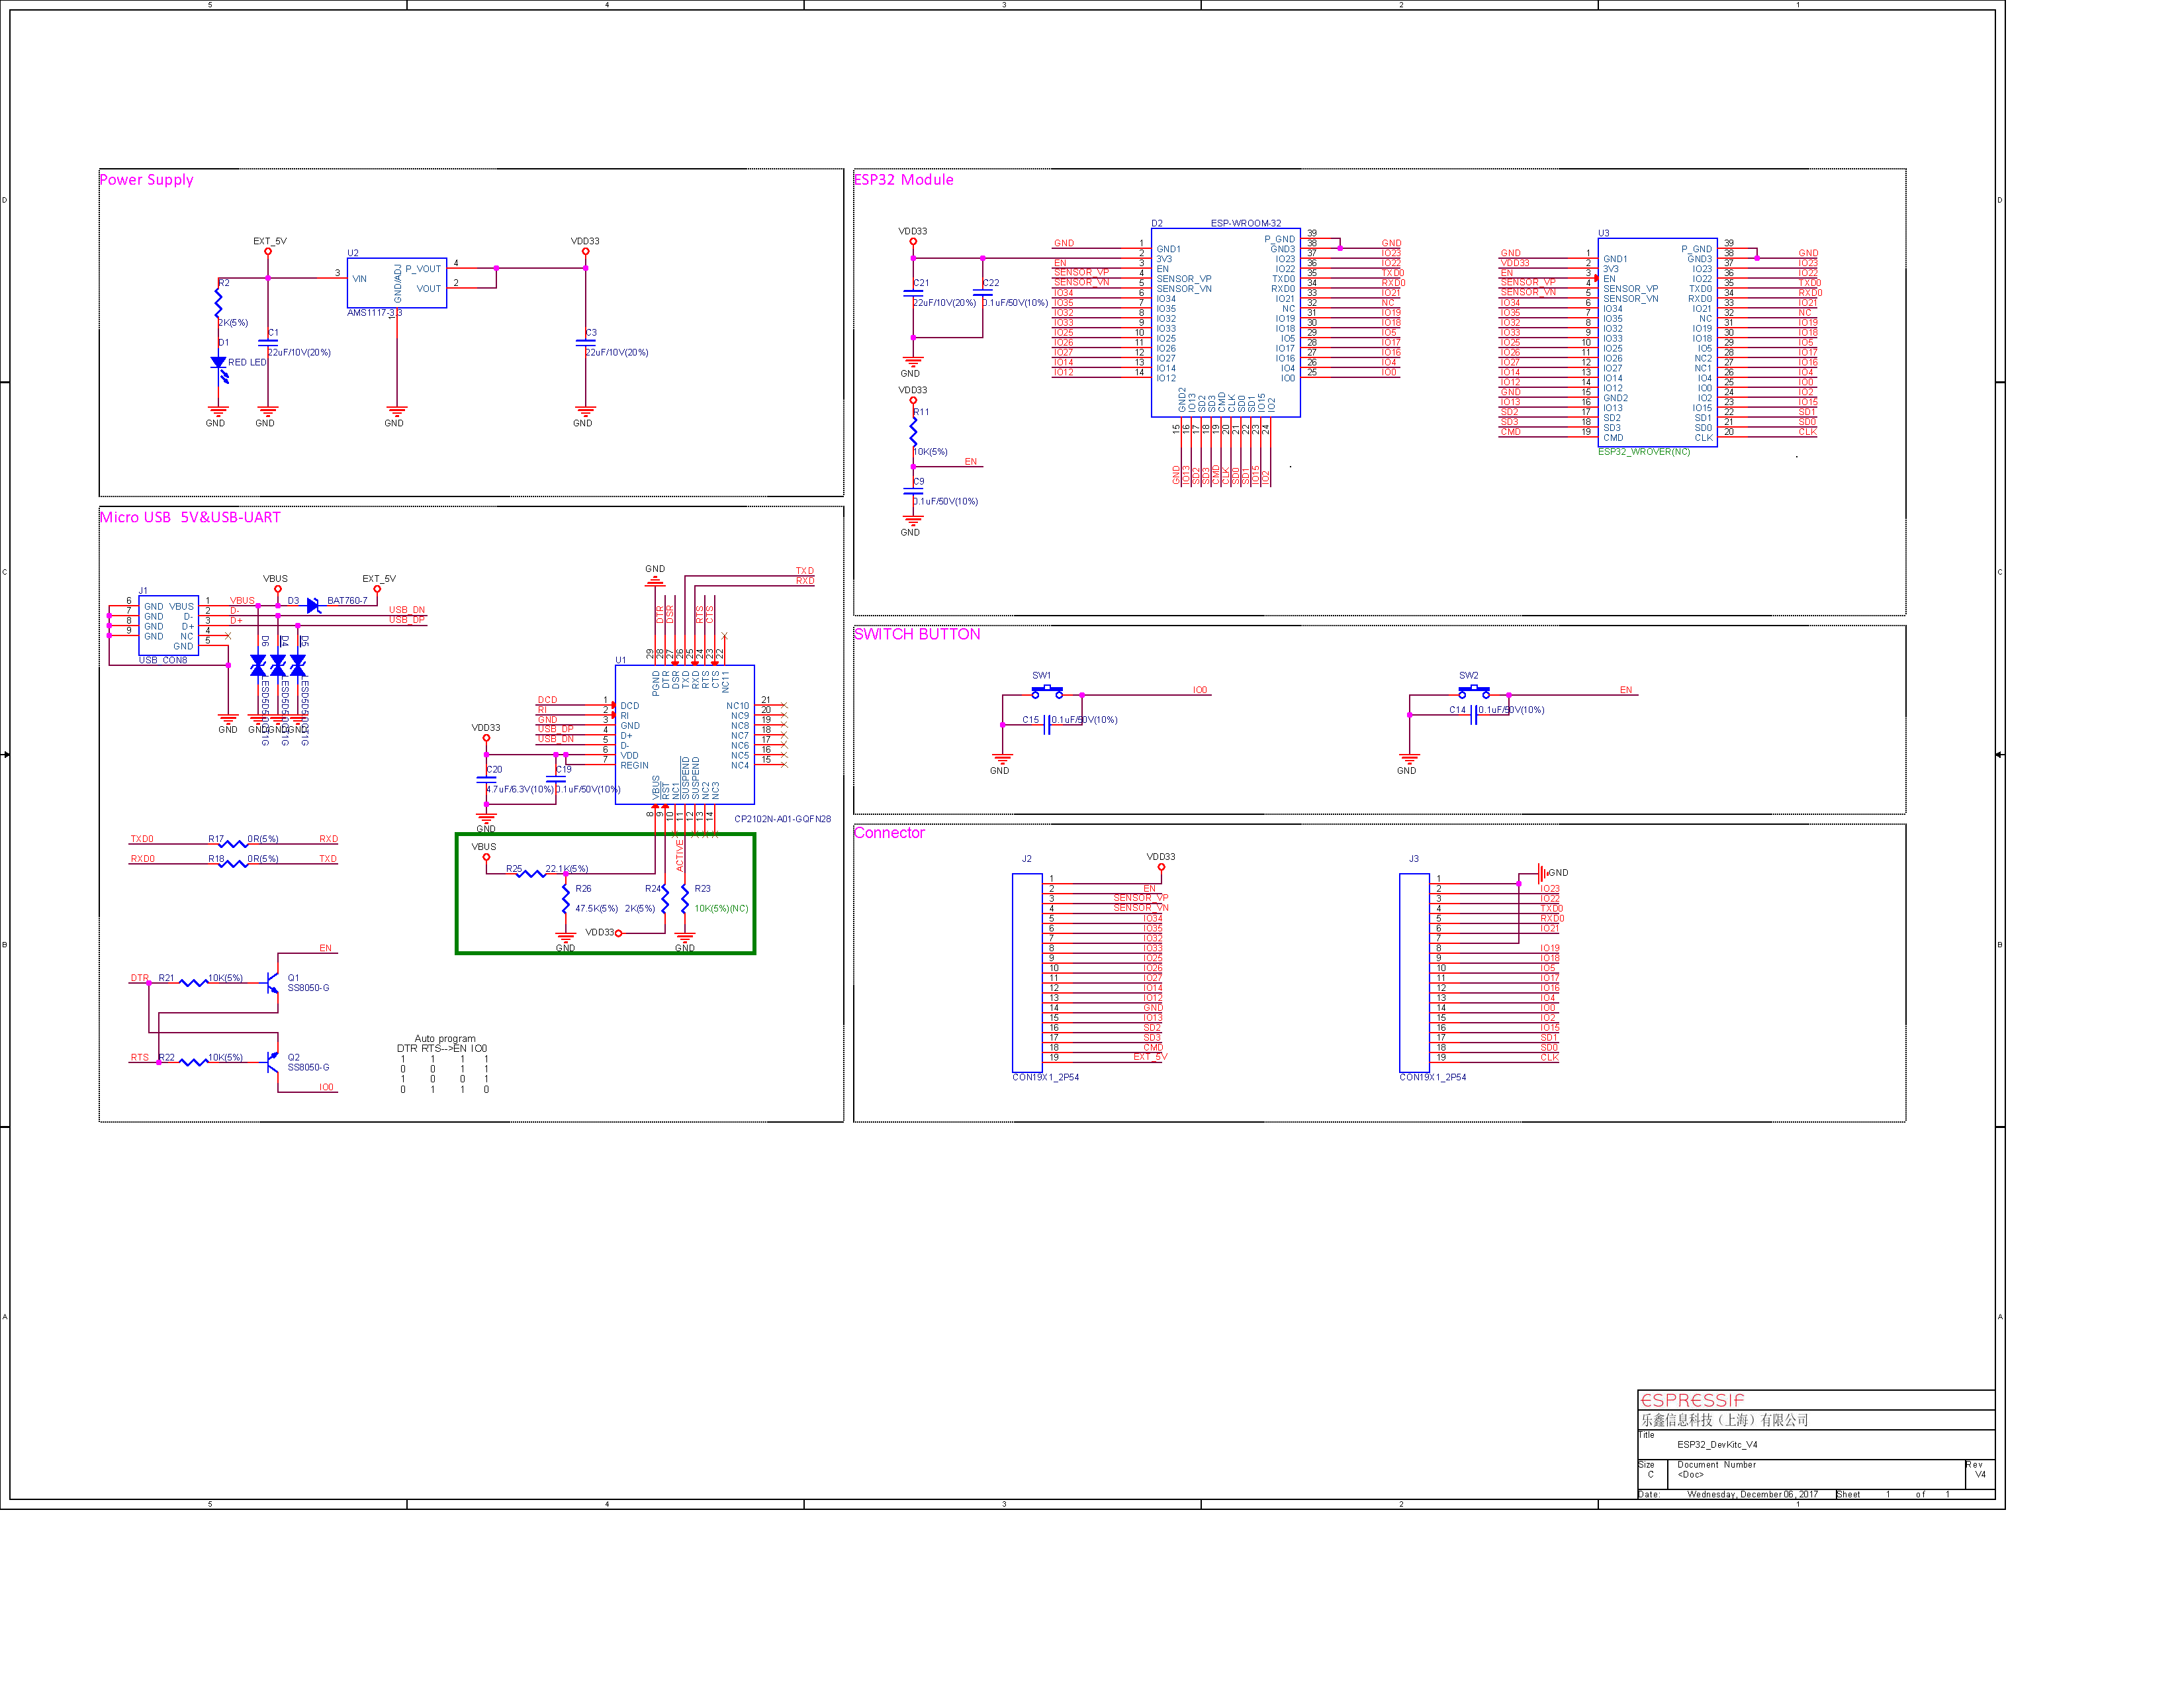
\includepdf[pages=1, angle=90]{ane_esp_kit/esp32_devkitc_v4-sch.pdf}
\end{landscape}
\chapter[Esquema módulo ESP]{Desenho Esquemático Módulo ESP32-WROOM-32E}

\label{ane:mod}

\begin{landscape}
    \begin{figure}[htb]
        \begin{center}
            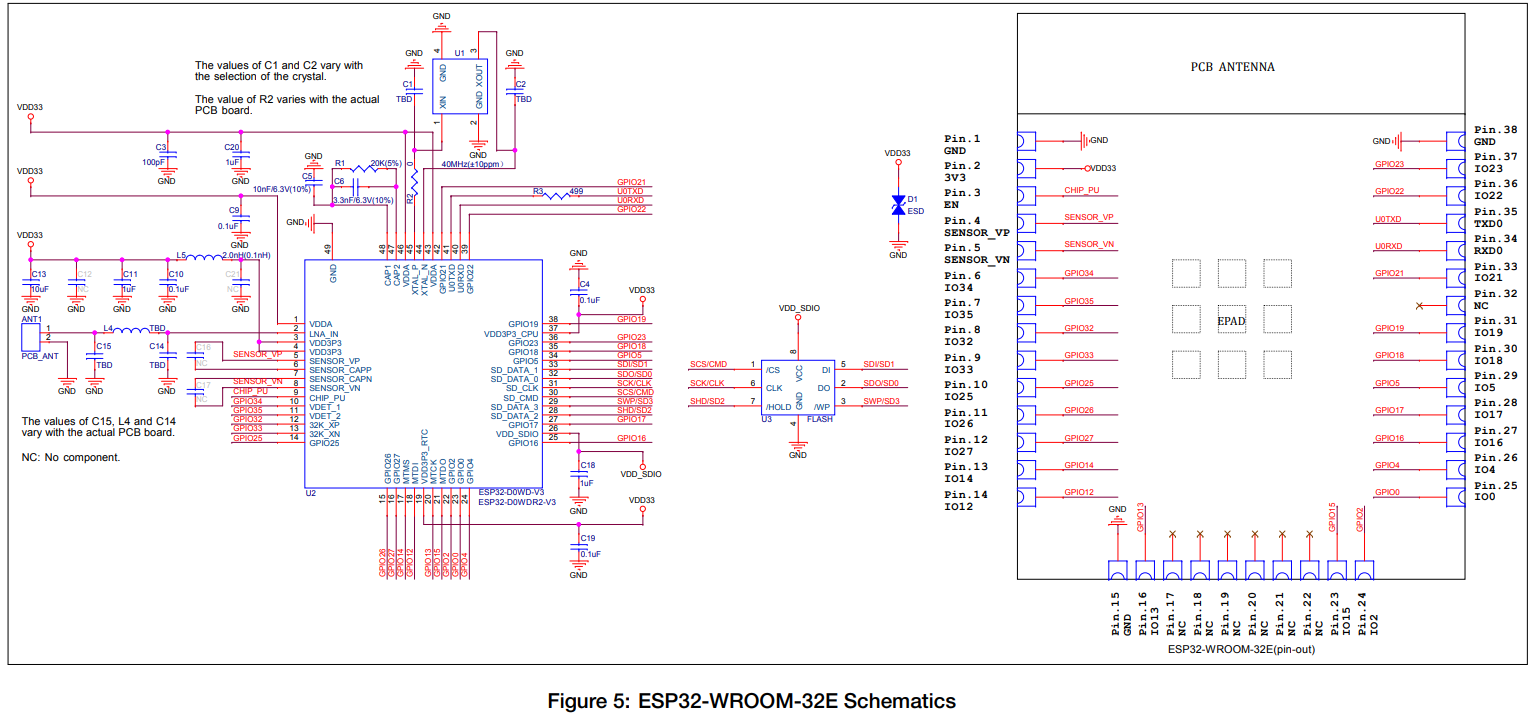
\includegraphics[scale=0.5]{ane_esp_mod/mod-esq.png}
        \end{center}
    \end{figure}
\end{landscape}
    

\end{anexosenv}


\end{document}